% Options for packages loaded elsewhere
\PassOptionsToPackage{unicode}{hyperref}
\PassOptionsToPackage{hyphens}{url}
\PassOptionsToPackage{dvipsnames,svgnames,x11names}{xcolor}
%
\documentclass[
  10pt,
]{article}
\usepackage{amsmath,amssymb}
\usepackage{iftex}
\ifPDFTeX
  \usepackage[T1]{fontenc}
  \usepackage[utf8]{inputenc}
  \usepackage{textcomp} % provide euro and other symbols
\else % if luatex or xetex
  \usepackage{unicode-math} % this also loads fontspec
  \defaultfontfeatures{Scale=MatchLowercase}
  \defaultfontfeatures[\rmfamily]{Ligatures=TeX,Scale=1}
\fi
% lmodern omitted
\ifPDFTeX\else
  % xetex/luatex font selection
  \setmainfont[]{DejaVu Serif}
  \setsansfont[]{DejaVu Sans}
  \setmonofont[]{DejaVu Sans Mono}
  \setmathfont[]{DejaVu Math TeX Gyre}
\fi
% Use upquote if available, for straight quotes in verbatim environments
\IfFileExists{upquote.sty}{\usepackage{upquote}}{}
\IfFileExists{microtype.sty}{% use microtype if available
  \usepackage[]{microtype}
  \UseMicrotypeSet[protrusion]{basicmath} % disable protrusion for tt fonts
}{}
\makeatletter
\@ifundefined{KOMAClassName}{% if non-KOMA class
  \IfFileExists{parskip.sty}{%
    \usepackage{parskip}
  }{% else
    \setlength{\parindent}{0pt}
    \setlength{\parskip}{6pt plus 2pt minus 1pt}}
}{% if KOMA class
  \KOMAoptions{parskip=half}}
\makeatother
\usepackage{xcolor}
\usepackage[margin=2.2cm]{geometry}
\usepackage{longtable,booktabs,array}
\usepackage{calc} % for calculating minipage widths
% Correct order of tables after \paragraph or \subparagraph
\usepackage{etoolbox}
\makeatletter
\patchcmd\longtable{\par}{\if@noskipsec\mbox{}\fi\par}{}{}
\makeatother
% Allow footnotes in longtable head/foot
\IfFileExists{footnotehyper.sty}{\usepackage{footnotehyper}}{\usepackage{footnote}}
\makesavenoteenv{longtable}
\usepackage{graphicx}
\makeatletter
\def\maxwidth{\ifdim\Gin@nat@width>\linewidth\linewidth\else\Gin@nat@width\fi}
\def\maxheight{\ifdim\Gin@nat@height>\textheight\textheight\else\Gin@nat@height\fi}
\makeatother
% Scale images if necessary, so that they will not overflow the page
% margins by default, and it is still possible to overwrite the defaults
% using explicit options in \includegraphics[width, height, ...]{}
\setkeys{Gin}{width=\maxwidth,height=\maxheight,keepaspectratio}
% Set default figure placement to htbp
\makeatletter
\def\fps@figure{htbp}
\makeatother
\setlength{\emergencystretch}{3em} % prevent overfull lines
\providecommand{\tightlist}{%
  \setlength{\itemsep}{0pt}\setlength{\parskip}{0pt}}
\setcounter{secnumdepth}{-\maxdimen} % remove section numbering
\ifLuaTeX
\usepackage[bidi=basic]{babel}
\else
\usepackage[bidi=default]{babel}
\fi
\babelprovide[main,import]{czech}
\ifPDFTeX
\else
\babelfont{rm}[]{DejaVu Serif}
\fi
% get rid of language-specific shorthands (see #6817):
\let\LanguageShortHands\languageshorthands
\def\languageshorthands#1{}
\usepackage{caption}
\captionsetup{labelformat=empty,font=small}
\usepackage{float}
\floatplacement{figure}{H}
\usepackage{needspace}
\usepackage{etoolbox}
\pretocmd{\section}{\Needspace{10\baselineskip}}{}{}
\pretocmd{\subsection}{\Needspace{7\baselineskip}}{}{}
\usepackage{lastpage}
\usepackage{fancyhdr}
\fancypagestyle{plain}{\fancyhf{}\renewcommand{\headrulewidth}{0pt}\fancyfoot[C]{\small\thepage\,/\,\pageref*{LastPage}}}
\pagestyle{plain}
\widowpenalty=10000
\clubpenalty=10000
\renewcommand{\abstractname}{Abstrakt}
\ifLuaTeX
  \usepackage{selnolig}  % disable illegal ligatures
\fi
\IfFileExists{bookmark.sty}{\usepackage{bookmark}}{\usepackage{hyperref}}
\IfFileExists{xurl.sty}{\usepackage{xurl}}{} % add URL line breaks if available
\urlstyle{same}
\hypersetup{
  pdftitle={Nízko položené nuly 795 381 kvadratických Dirichletových L-funkcí do vodiče 10\^{}\{10\}: domněnka poměrů, souvislé rodiny a první nula --- reprodukovatelná numerická studie III},
  pdfauthor={David Hess (MAYAN ALFA V1008 LAB v.34.68e)},
  pdflang={cs},
  colorlinks=true,
  linkcolor={Maroon},
  filecolor={Maroon},
  citecolor={Blue},
  urlcolor={Blue},
  pdfcreator={LaTeX via pandoc}}

\title{Nízko položené nuly 795 381 kvadratických Dirichletových L-funkcí
do vodiče \(10^{10}\): domněnka poměrů, souvislé rodiny a první nula ---
reprodukovatelná numerická studie III}
\author{David Hess (MAYAN ALFA V1008 LAB v.34.68e)}
\date{5.11.2026}

\begin{document}
\maketitle
\begin{abstract}
Třetí studie této řady přechází od Riemannovy funkce zeta k rodině
L-funkcí. Pro 795 381 kvadratických Dirichletových L-funkcí
\(L(s, \chi_D)\) --- jedenáct rodin základních diskriminantů od
\(|D| \approx 10^3\) do \(10^{10}\), mezi nimi všechny diskriminanty s
\(10^6 < |D| \le 2\cdot10^6\) a 60 000 náhodně vybraných --- byly nízko
položené nuly spočteny programem PARI/GP nezávisle na dvou počítačích;
69 452 L-funkcí spočtených na obou má nuly totožné. Jednohladinová
hustota rozvinutých nul se srovnává s limitou Katze a Sarnaka USp, s
konečnou maticí USp\((2N)\) a s domněnkou poměrů Conreyho, Farmera a
Zirnbauera v podobě Conreyho a Snaithové (2007), vyčíslenou pro každý
diskriminant bez volného parametru. Domněnka poměrů popíše všechny
rodiny (\(\chi^2\) na koš 0,54--1,19 proti asi 0,95 očekávaným pro
nezávislé L-funkce; hustota u středového bodu v rodině 607 941 L-funkcí
\(0{,}6082 \pm 0{,}0014\) proti \(0{,}6084\)), kdežto limita USp dává
\(\chi^2\) na koš 5 až 850 v rodinách aspoň 6 000 L-funkcí a ještě při
\(|D| = 10^{10}\) je vzdálena o 12 směrodatných chyb. Rodiny po sobě
jdoucích diskriminantů mají \(\chi^2\) pod hodnotou pro nezávislé
L-funkce; kosinový rozklad odchylek ukazuje, že schodek leží celý na
nízkých frekvencích (\(u < 1\) v rozvinuté proměnné): pásma 6 074 po
sobě jdoucích diskriminantů mají 0,23, 0,36 a 0,48 výkonu náhodných
výběrů na nízkých frekvencích při \(|D| \approx 5\cdot10^4\),
\(1{,}5\cdot10^6\) a \(10^8\) (5,9, 10,2 a 4,3 směrodatné chyby), na
vysokých frekvencích bez rozdílu. Jev plyne z explicitního vzorce: v
úseku po sobě jdoucích diskriminantů procházejí průměry \(\chi_D(p)\)
pro prvočísla menší než délka úseku téměř úplné periody; podmnožiny
složené z \(m\) kratších kusů jev se vzrůstajícím \(m\) postupně
ztrácejí, kdežto vyrovnání zbytkových tříd \(D\) --- testované pro 19
modulů od 3 do 840 včetně prvočísla 131 a pro samotné znaménko, s
nezávislým opakováním --- ho nevytvoří. Bez použití nul seřadí zbylý
rozptyl součtů \(\chi_D(p)\) přes podmnožinu výkon nul na nízkých
frekvencích všech 60 stratifikovaných podmnožin a souvislých pásem podél
přímky dané náhodnými výběry a pásmy; velikost souhlasí jen na hraně
(\(\chi^2 = 82{,}05\) pro 60 bodů se společnými chybami), stratifikace
sníží výkon o něco méně, než přímka předpoví. Nízká hodnota
\(\chi^2 = 0{,}54\) rodiny \(10^4 < |D| \le 2\cdot10^4\) je nejnižší z
devíti takových pásem, 1,5 směrodatné odchylky pod jejich průměrem. Pro
první nulu selhává USp\((2N)\) s \(N = \frac12\ln(|D|/\pi)\), kdežto
USp\((2N_{\mathrm{ef}})\) s \(N_{\mathrm{ef}}\) určeným domněnkou poměrů
dává pro liché charaktery celé rozdělení v mezích chyb při každém
vodiči; pro sudé charaktery leží první nula výš o člen nižšího řádu,
který klesá zhruba jako \(0{,}094/\ln(|D|/\pi)\). Očekávaný výkon
nízkých frekvencí jakéhokoli způsobu výběru podmnožiny vychází bez
losování, když se chyba vezme z očekávaného počtu modelu (jako ve studii
II); losuje se jen malý zbylý rozdíl, což chybu zmenší asi čtyřikrát. Už
trojice po sobě jdoucích diskriminantů leží pod náhodným výběrem (B10:
0,972 náhodné hodnoty, 4,7 chyby); dřívější posun o několik procent mezi
testem a touto přesnou hodnotou je zkreslení chyby z pozorovaného počtu
ve dvou nejnižších koších, ne šum; výběry vyvážené na \(\chi_D(p)\) pro
všechna \(p \le P\) dosáhnou hladiny, kterou předpoví regrese příspěvku
každé L-funkce na \(\chi_D(p)\). Kosinové módy \(k\) a \(8 - k\) jedné
L-funkce jsou spřažené (korelace 0,35--0,58, pro poissonovské nuly 0) a
součiny \(\chi_D(p)\chi_D(q)\) malých prvočísel nesou módy 6--7 (14× až
19× víc než módy 1--4). U sudých charakterů protne rozdělení první nuly
USp\((2N_{\mathrm{ef}})\) v C100 v \(x_1 = 0{,}508 \pm 0{,}021\); test
kalibrace ukazuje, že tento bod sleduje konec intervalu
\([0, \frac12]\), na kterém se \(N_{\mathrm{ef}}\) určuje, a není
vlastností nul. Přepočet každého losovaného čísla oddílů 4.3--4.5 tímto
principem, se stejnými pravidly a návrhy, závěry drží a tři zpřesní
(oddíl 4.7): stratifikace výkon nízkých frekvencí ve všech třech velkých
rodinách skutečně snižují (\(D \bmod 840\): 26,6, 13,5 a 2,9 směrodatné
chyby), ale jen o 0,89, 0,56 a 0,39 toho, co dává přímka mezi náhodnými
výběry a pásmy, takže přímka je ve velikosti zamítnuta
(\(\chi^2 = 841{,}8\) pro 60); váhy explicitní formule reprodukují
regresi jednotlivých L-funkcí na \(\chi_D(p)\) jen spolu s duálním
členem domněnky poměrů (sklon 0,995--0,999 místo 0,52--0,60); a posun
průměru první nuly sudých charakterů závisí na intervalu, na kterém se
\(N_{\mathrm{ef}}\) určuje, a pro \([0; 0{,}7]\) je nejvýš 0,004, kdežto
odchylka jejího tvaru ve dvou rodinách zůstává. Zvětšení rodiny u
\(|D| = 10^{10}\) na 121 557 L-funkcí (oddíl 4.8) zachová všechny
výsledky s asi třikrát menšími chybami; jev souvislých rodin trvá (0,62
výkonu náhodných výběrů) a člen sudých charakterů u první nuly klesá
rychleji než \(1/\ln(|D|/\pi)\). Data a skripty reprodukují každé číslo,
s nezávislou kontrolou; o zobecněné Riemannově hypotéze nic neříkají.
\end{abstract}

\hypertarget{uxfavod}{%
\section{1. Úvod}\label{uxfavod}}

První dvě studie této řady {[}1, 2{]} srovnávaly statistiku nul
Riemannovy funkce zeta se vzorci Berryho, Bogomolného a Keatinga, v
nichž vystupují prvočísla jako periodické orbity. Berry a Keating
{[}3{]} svůj přehled uzavírají rodinami L-funkcí, pro které Katz a
Sarnak {[}4, 5{]} předpověděli, že nuly u středového bodu sledují jednu
z klasických kompaktních grup: pro kvadratické Dirichletovy L-funkce
\(L(s, \chi_D)\), \(\chi_D(n) = (D/n)\), unitární symplektickou grupu
USp. Özlük a Snyder {[}6{]} a Rubinstein {[}7{]} dokázali
jednohladinovou hustotu této rodiny pro testovací funkce s omezeným
nosičem a Rubinstein {[}7{]} ji srovnal s numerickými nulami. Přiblížení
k limitě je pomalé: při konečném vodiči je hustota u středového bodu
výrazně nad hodnotou USp a členy nižšího řádu dává domněnka poměrů
Conreyho, Farmera a Zirnbauera {[}8{]} v podobě, kterou propracovali
Conrey a Snaithová {[}9{]}; Miller {[}10{]} ji pro tuto rodinu testoval.

Tato studie měří tato tvrzení na jedenácti rodinách kvadratických
L-funkcí od \(|D| \approx 10^3\) do \(10^{10}\) (oddíl 2):
jednohladinovou hustotu proti domněnce poměrů a nulovým modelům (4.1),
pomalé přiblížení k USp (4.2), otázku, proč rodiny po sobě jdoucích
diskriminantů dávají \(\chi^2\) pod hodnotou nezávislých L-funkcí (4.3),
zda ho vytvoří vyrovnání zbytkových tříd a jak ho bez nul předpoví
součty charakterů (4.4), a rozdělení první nuly (4.5). Domněnka poměrů,
limita Katze a Sarnaka i efektivní velikost matice {[}11, 12{]} jsou
známé; přínosem je soustavný, reprodukovatelný test na 795 381
L-funkcích s nulovými modely a nezávislou kontrolou, mechanismus nízkého
\(\chi^2\) souvislých rodin změřený podle frekvencí a předpovězený ze
součtů charakterů a rozdílné chování sudých a lichých charakterů u první
nuly. Oddíl 6 odděluje, co je nové a co potvrzené.

\hypertarget{data}{%
\section{2. Data}\label{data}}

{\small\begin{longtable}[]{@{}
  >{\raggedright\arraybackslash}p{(\columnwidth - 8\tabcolsep) * \real{0.0857}}
  >{\raggedright\arraybackslash}p{(\columnwidth - 8\tabcolsep) * \real{0.4286}}
  >{\raggedleft\arraybackslash}p{(\columnwidth - 8\tabcolsep) * \real{0.1571}}
  >{\raggedleft\arraybackslash}p{(\columnwidth - 8\tabcolsep) * \real{0.1571}}
  >{\raggedright\arraybackslash}p{(\columnwidth - 8\tabcolsep) * \real{0.1714}}@{}}
\toprule\noalign{}
\begin{minipage}[b]{\linewidth}\raggedright
rodina
\end{minipage} & \begin{minipage}[b]{\linewidth}\raggedright
diskriminanty
\end{minipage} & \begin{minipage}[b]{\linewidth}\raggedleft
L-funkcí
\end{minipage} & \begin{minipage}[b]{\linewidth}\raggedleft
nul
\end{minipage} & \begin{minipage}[b]{\linewidth}\raggedright
spočteno na
\end{minipage} \\
\midrule\noalign{}
\endhead
\bottomrule\noalign{}
\endlastfoot
A & všechny s \(10^3 < |D| \le 3\cdot10^3\) & 1 213 & 5 209 & počítač
1 \\ \addlinespace[2pt]
B & \(10^4 < |D| \le 2\cdot10^4\) & 6 074 & 26 355 & počítač 1 \\ \addlinespace[2pt]
B10 & \(10^4 < |D| \le 10^5\) (obsahuje B) & 54 700 & 237 553 & počítač
1 \\ \addlinespace[2pt]
C10 & \(10^6 < |D| \le 1{,}1\cdot10^6\) & 60 795 & 264 063 & počítač
1 \\ \addlinespace[2pt]
C100 & \(10^6 < |D| \le 2\cdot10^6\) (obsahuje C10) & 607 941 & 2 639
990 & počítač 2 \\ \addlinespace[2pt]
D10 & \(10^8 < |D| \le 10^8 + 10^4\) & 6 081 & 26 311 & počítač 1 \\ \addlinespace[2pt]
D100 & \(10^8 < |D| \le 10^8 + 10^5\) (obsahuje D10) & 60 802 & 263 065
& počítač 2 \\ \addlinespace[2pt]
E & \(10^{10} < |D| \le 10^{10} + 2\cdot10^3\) & 1 206 & 5 201 & počítač
1 \\ \addlinespace[2pt]
E10 & \(10^{10} < |D| \le 10^{10} + 2\cdot10^4\) (obsahuje E) & 12 153 &
52 355 & počítač 2 \\ \addlinespace[2pt]
R & 6 000 náhodných, \(10^6 \le |D| < 10^7\) (semínko 3462) & 6 000 & 26
031 & počítač 1 \\ \addlinespace[2pt]
R10 & 60 000 náhodných, \(10^6 \le |D| < 10^7\) (semínko 34620) & 60 000
& 260 183 & počítač 2 \\ \addlinespace[2pt]
\end{longtable}}

\(D\) probíhá základní diskriminanty obou znamének; \(D > 0\) dává sudý
charakter, \(D < 0\) lichý. Celkem 795 381 různých L-funkcí s 3 452 121
nulami (876 965 L-funkcí a 3 806 316 nul po rodinách, s překryvy). Nuly
spočetl jediný skript \texttt{ks\_nuly.py} (PARI/GP 2.17.2 {[}13{]},
\texttt{lfuncreate} a \texttt{lfunzeros}) do rozvinuté výšky
\(x = 4{,}3\), asi čtyři nuly na L-funkci, a uložil je po blocích se
SHA-256; náhodné rodiny používají pevný generátor splitmix64. Sady C100,
D100, E10 a R10 spočetl počítač 2 (macOS, 9 procesů, asi 33
procesorových hodin), ostatní počítač 1 (Linux, 2 procesy). Všech 68 082
diskriminantů rodin C10, D10 a E a 1 370 diskriminantů, které náhodné
rodiny sdílejí s rodinami druhého počítače, má nuly totožné do
posledního uloženého místa; B je totožná uvnitř B10. Kontrola bez PARI
potvrzuje pro každou rodinu, že každý základní diskriminant je v ní
právě jednou (vlastní síto bezčtvercovosti) a že nuly jsou kladné a
rostoucí; u 40 L-funkcí pěti velkých rodin se počet změn znaménka
Hardyho funkce (\texttt{lfunhardy}, jiná funkce PARI) na jemné mřížce
rovná počtu uložených nul. Samotné nuly nejsou součástí publikace;
generátor, manifesty a SHA-256 rozbaleného obsahu každého bloku ano.

\hypertarget{metody}{%
\section{3. Metody}\label{metody}}

\textbf{Rozvinutí.} Pro doplněnou funkci
\((|D|/\pi)^{s/2}\Gamma((s + \kappa)/2) L(s, \chi_D)\), \(\kappa = 0\)
pro \(D > 0\) a \(\kappa = 1\) pro \(D < 0\), se nuly
\(\frac12 + i\gamma\) rozvinou jako \(x = \theta_D(\gamma)/\pi\), kde
\[\theta_D(t) = \frac{t}{2}\ln\frac{|D|}{\pi} + \operatorname{Im}\ln\Gamma\!\left(\frac{1/2 + \kappa}{2} + \frac{it}{2}\right),\]
takže střední hustota je 1. Pro každou L-funkci se uchovává histogram
\(x\) po koších 0,025 do \(x = 4\).

\textbf{Modely.} Limita Katze a Sarnaka je
\(W_{\mathrm{USp}}(x) = 1 - \sin(2\pi x)/(2\pi x)\). Konečná matice
USp\((2N)\) s \(N = \frac12 l\), \(l = \ln(|D|/\pi)\), má
\(W_N(x) = 1 + \frac{1}{2N} - \sin((2N + 1)\pi x/N)/(2N\sin(\pi x/N))\).
Domněnka poměrů {[}8, 9{]} dává hustotu nul v \(t\) pro jeden
diskriminant
\[\rho_D(t) = \frac{\theta_D'(t)}{\pi} + \frac{1}{\pi}\operatorname{Re}\left[\frac{\zeta'}{\zeta}(1 + 2it) + A'(it) - \left(\frac{|D|}{\pi}\right)^{-it}\frac{\Gamma(\frac14 + \frac\kappa2 - \frac{it}{2})}{\Gamma(\frac14 + \frac\kappa2 + \frac{it}{2})}\,\zeta(1 - 2it)\,A(it)\right],\]
\[A(it) = \prod_p\left(1 - \frac{p^{2it} - 1}{p^2 - 1}\right), \qquad A'(it) = \sum_p \frac{\ln p}{(p + 1)(p^{1 + 2it} - 1)},\]
s aritmetickými činiteli rodiny všech základních diskriminantů (podíl
\(D\) dělitelných \(p\) je \(1/(p + 1)\)). Je to tvar Conreyho a
Snaithové {[}9, věta 3.1{]} přizpůsobený této rodině; pro liché
charaktery s činitelem \(\Gamma(\frac34 \pm \frac{it}{2})\) jde o naši
analogii. Předpověď pro rodinu je průměr \(\rho_D\) přes všechny její
diskriminanty, vyčíslený na mřížce v \(t\) s krokem 0,002 (mpmath, 30
míst; prvočísla do \(2\cdot10^5\)) a lineárně interpolovaný v \(l\) mezi
uzly vzdálenými 0,002; póly v \(t = 0\) se ruší. Nulový model vynechá
\(A\) i \(A'\).

\textbf{Statistika.} Pro koše šířky 0,025, 0,05 a 0,1 se \(\chi^2\) na
koš počítá s Poissonovou chybou pozorovaného počtu (Neymanův tvar; oddíl
4.6 jej srovnává s Pearsonovým tvarem, který bere chybu z očekávaného
počtu modelu jako studie II). Protože se nuly jedné L-funkce navzájem
odpuzují, kolísá počet v koši mezi L-funkcemi méně než Poissonova
veličina; nezávislé L-funkce kolem přesného modelu by daly \(\chi^2\) na
koš asi 0,95, spočtené z druhých mocnin počtů. Bootstrap přes L-funkce
(200 převzorkování s vracením) dává pás \(\chi^2\) ze samotného
výběrového šumu a pravděpodobnost hodnoty tak malé jako naměřená; test
bez košů používá největší odchylku kumulativního počtu.

\textbf{Podmnožiny.} K testu rodin po sobě jdoucích diskriminantů se
B10, C100 a D100 rozdělí na pásma 6 074 po sobě jdoucích diskriminantů
(podle \(|D|\); velikost rodiny B) a srovnají s náhodnými výběry téže
velikosti z téže rodiny a s náhodnými výběry se stejným zastoupením tříd
(znaménko, \(D \bmod M\)), \(M = 8, 24, 120, 840\), jako celá rodina
(oddíl 4.4 to rozšíří na 19 modulů a na samotné znaménko, \(M = 1\)).
Pro každou podmnožinu se 80 odchylek
\(r_b = (\text{data} - \text{předpověď})/\text{chyba}\) po koších 0,05
rozloží ortonormální kosinovou transformací
\(c_k = \sum_b \sqrt{(2 - \delta_{k0})/80}\,\cos(\pi k(b + \frac12)/80)\,r_b\);
\(\chi^2\) na koš je \(\sum_k c_k^2/80\) a index \(k\) je frekvence
\(u = k/8\) v \(x\). V testu kusy se podmnožina 6 074 diskriminantů
složí z \(m\) souvislých kusů na náhodných místech (\(m = 1\): jeden
úsek; \(m = 6074\): náhodný výběr). Každý průměr přes náhodné podmnožiny
se uvádí s chybou, směrodatnou odchylkou podmnožin dělenou odmocninou
jejich počtu.

\textbf{Součty charakterů.} Pro každý typ podmnožiny se rozptyl \(V_p\)
průměru \(\langle\chi_D(p)\rangle_{\mathcal S}\) přes podmnožinu
(vlastní Kroneckerův symbol, Eulerovo kritérium) srovná s rozptylem
\(\sigma_p^2/N\,(1 - N/n)\) náhodného výběru \(N\) z rodiny \(n\) prvků.
Pro stratifikaci se počítá přesně, bez losování: když se \(k_c\) z \(N\)
prvků vybírá bez vracení ze třídy \(c\) velikosti \(n_c\) s průměrem
\(m_c\) a výběrovým rozptylem \(S_c^2\), je
\(V_p = \sum_c k_c(1 - k_c/n_c)S_c^2/N^2 + (\sum_c k_c m_c/N - \mu_p)^2\);
300 losování na typ potvrdí, že náhodné výběry sledují konečný soubor.
Podíl, který podmnožina zachová,
\(W = \sum_p w_p V_p(\mathcal S)/\sum_p w_p \sigma_p^2/N\,(1 - N/n)\) s
vahou \(w_p = (\ln p)^2/p\) explicitního vzorce, se bere přes
\(p \le 100\) (\(W_{100}\)) nebo přes všechna prvočísla nízkých módů,
\(p \le e^{7L/8}\) (\(W_E\)). Pro souvislá pásma se poměr
\(r_p = V_p(\text{pásma})/(\sigma_p^2/N\,(1 - N/n))\) počítá pro 582
prvočísel do \(4\cdot10^6\) (vektorový Jacobiho symbol). Přímka dvěma
body rodiny --- náhodnými výběry při \(W = 1\) a souvislými pásmy při
jejich \(W\) --- předpoví výkon na nízkých frekvencích každé
stratifikace, aniž se ke stratifikacím něco prokládá; její \(\chi^2\)
bere v úvahu, že oba body jsou společné všem stratifikacím rodiny
(kovarianční matice).

\textbf{První nula.} Rozdělení první rozvinuté nuly \(x_1\) se srovnává
s \(1 - E(0, s)\), \(E(0, s) = \det(I - K)\) na \([0, s]\) s jádrem
\(S_N(x - y) - S_N(x + y)\),
\(S_N(z) = \sin((2N + 1)\pi z/(2N))/(2N\sin(\pi z/(2N)))\)
(Gauss--Legendre, 40 uzlů; limita USp s \(S(z) = \sin(\pi z)/(\pi z)\)).
Vedle \(N = \frac12 l\) se používá efektivní \(N_{\mathrm{ef}}\),
zvolené tak, aby hustota USp\((2N_{\mathrm{ef}})\) v \([0, \frac12]\)
byla rovna hustotě domněnky poměrů pro tutéž rodinu --- z teorie, ne z
nul --- v duchu efektivní velikosti matice Bogomolného a kol. {[}11{]}
pro \(\zeta\) a Dueñeze a kol. {[}12{]} pro eliptické křivky.
Kolmogorovovy--Smirnovovy vzdálenosti jsou uvedeny s kritickou hodnotou
\(1{,}36/\sqrt n\).

\hypertarget{vuxfdsledky}{%
\section{4. Výsledky}\label{vuxfdsledky}}

\hypertarget{jednohladinovuxe1-hustota-proti-domnux11bnce-pomux11brux16f}{%
\subsection{4.1 Jednohladinová hustota proti domněnce
poměrů}\label{jednohladinovuxe1-hustota-proti-domnux11bnce-pomux11brux16f}}

\begin{figure}
\centering
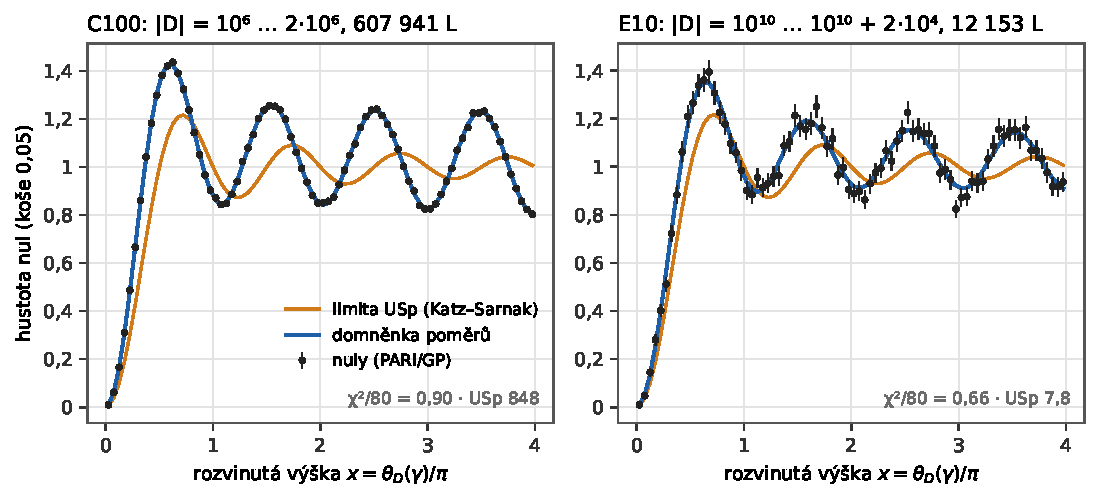
\includegraphics[width=0.95\textwidth,height=\textheight]{../../figures/01_density_cz.pdf}
\caption{Obrázek 1. Hustota rozvinutých nul po koších 0,05 v rodinách
C100 (vlevo) a E10 (vpravo) proti domněnce poměrů (modře) a limitě Katze
a Sarnaka USp (oranžově).}
\end{figure}

{\small\begin{longtable}[]{@{}
  >{\raggedright\arraybackslash}p{(\columnwidth - 8\tabcolsep) * \real{0.0896}}
  >{\raggedleft\arraybackslash}p{(\columnwidth - 8\tabcolsep) * \real{0.1194}}
  >{\raggedright\arraybackslash}p{(\columnwidth - 8\tabcolsep) * \real{0.2687}}
  >{\raggedleft\arraybackslash}p{(\columnwidth - 8\tabcolsep) * \real{0.1642}}
  >{\raggedright\arraybackslash}p{(\columnwidth - 8\tabcolsep) * \real{0.3582}}@{}}
\toprule\noalign{}
\begin{minipage}[b]{\linewidth}\raggedright
rodina
\end{minipage} & \begin{minipage}[b]{\linewidth}\raggedleft
\(\ln|D|\)
\end{minipage} & \begin{minipage}[b]{\linewidth}\raggedright
\(\chi^2\)/koš 0,05: poměry / bez \(A\) / USp
\end{minipage} & \begin{minipage}[b]{\linewidth}\raggedleft
\(p\) (bootstrap)
\end{minipage} & \begin{minipage}[b]{\linewidth}\raggedright
hustota v \([0; \frac12]\): data / poměry / USp
\end{minipage} \\
\midrule\noalign{}
\endhead
\bottomrule\noalign{}
\endlastfoot
A & 7,55 & 0,57 / 2,0 / 8,3 & \textless{} 0,005 &
\(0{,}772 \pm 0{,}036\) / 0,771 / 0,411 \\ \addlinespace[2pt]
B & 9,60 & 0,54 / 5,0 / 21 & \textless{} 0,005 & \(0{,}708 \pm 0{,}015\)
/ 0,702 / 0,411 \\ \addlinespace[2pt]
B10 & 10,77 & 0,87 / 33 / 142 & 0,34 & \(0{,}6718 \pm 0{,}0050\) /
0,6729 / 0,411 \\ \addlinespace[2pt]
C10 & 13,86 & 1,06 / 22 / 89 & 0,78 & \(0{,}6136 \pm 0{,}0045\) / 0,6134
/ 0,411 \\ \addlinespace[2pt]
C100 & 14,20 & 0,90 / 203 / 848 & 0,34 & \(0{,}6082 \pm 0{,}0014\) /
0,6084 / 0,411 \\ \addlinespace[2pt]
D10 & 18,42 & 0,98 / 1,8 / 5,1 & 0,60 & \(0{,}558 \pm 0{,}014\) / 0,560
/ 0,411 \\ \addlinespace[2pt]
D100 & 18,42 & 0,77 / 12 / 49 & 0,10 & \(0{,}5591 \pm 0{,}0043\) /
0,5595 / 0,411 \\ \addlinespace[2pt]
E & 23,03 & 0,71 / 0,80 / 1,2 & 0,04 & \(0{,}531 \pm 0{,}030\) / 0,527 /
0,411 \\ \addlinespace[2pt]
E10 & 23,03 & 0,66 / 2,6 / 7,8 & 0,02 & \(0{,}5273 \pm 0{,}0093\) /
0,5267 / 0,411 \\ \addlinespace[2pt]
R & 15,38 & 1,19 / 3,1 / 8,5 & 0,93 & \(0{,}609 \pm 0{,}014\) / 0,593 /
0,411 \\ \addlinespace[2pt]
R10 & 15,37 & 0,90 / 18 / 72 & 0,37 & \(0{,}5933 \pm 0{,}0044\) / 0,5925
/ 0,411 \\ \addlinespace[2pt]
\end{longtable}}

Domněnka poměrů popíše každou rodinu (obrázky 1 a 2): \(\chi^2\) na koš
0,54--1,19 při šířce koše 0,05, kde nezávislé L-funkce kolem přesného
modelu dávají 0,95 a pás bootstrapu je 0,70--1,24; nulové modely dávají
v největší rodině až 203 (bez aritmetického činitele) a 848 (USp).
Hustota v \([0; \frac12]\) souhlasí s domněnkou ve všech 33 kombinacích
rodiny a znaménka do 1,2 směrodatné chyby; v C100 je chyba 0,0014.
Souhlasí i počet nul do \(x = 4\) na L-funkci (C100: 4,0103 proti
4,0105; limita USp dává 3,756). Totéž platí pro šířky košů 0,025 a 0,1 i
bez košů (datové soubory). Několik rodin má \(\chi^2\) pod 0,95 ---
oddíl 4.3.

\begin{figure}
\centering
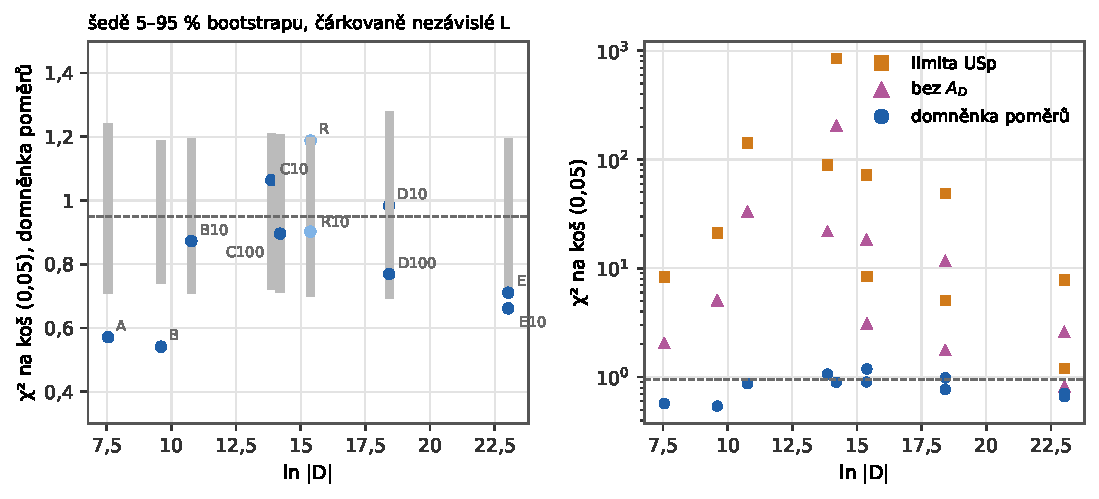
\includegraphics[width=0.95\textwidth,height=\textheight]{../../figures/02_chi2_families_cz.pdf}
\caption{Obrázek 2. Vlevo: \(\chi^2\) na koš (0,05) domněnky poměrů pro
všechny rodiny podle \(\ln|D|\) s pásem 5--95 \% bootstrapu (šedě) a
očekáváním pro nezávislé L-funkce (čárkovaně); náhodné rodiny světle
modře. Vpravo: totéž pro limitu USp a pro model bez aritmetického
činitele (logaritmicky).}
\end{figure}

\hypertarget{pux159ibluxedux17eenuxed-k-limitux11b-katze-a-sarnaka}{%
\subsection{4.2 Přiblížení k limitě Katze a
Sarnaka}\label{pux159ibluxedux17eenuxed-k-limitux11b-katze-a-sarnaka}}

\begin{figure}
\centering
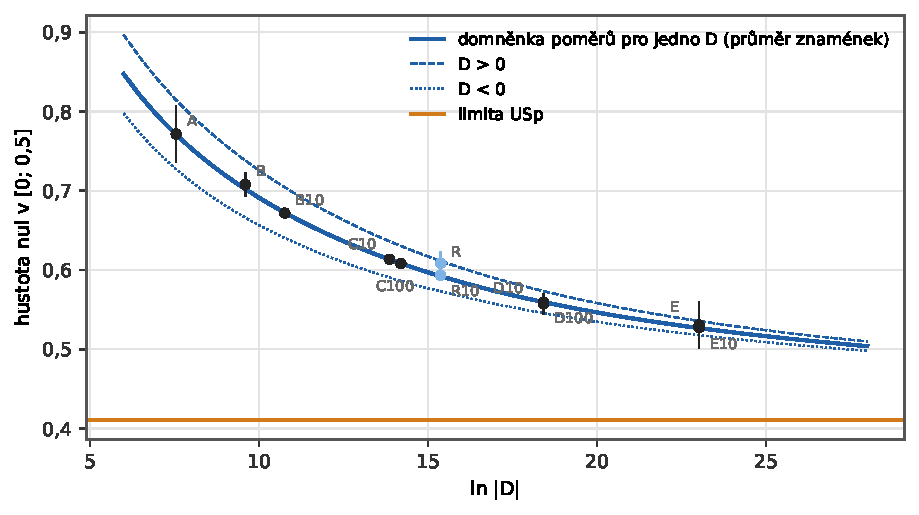
\includegraphics[width=0.8\textwidth,height=\textheight]{../../figures/03_approach_cz.pdf}
\caption{Obrázek 3. Hustota nul v \([0; \frac12]\) podle \(\ln|D|\):
rodiny (body), domněnka poměrů pro jeden diskriminant (čáry; průměr
znamének, \(D > 0\) čárkovaně, \(D < 0\) tečkovaně) a limita USp 0,411;
náhodné rodiny světle modře.}
\end{figure}

Hustota u středového bodu klesá z 0,772 při \(|D| \approx 2\cdot10^3\)
na 0,527 při \(10^{10}\) a sleduje domněnku poměrů pro jeden
diskriminant (obrázek 3), která hodnoty USp 0,411 dosahuje jen pomalu
(0,504 při \(\ln|D| = 28\)). Při \(|D| = 10^{10}\) dávají data
\(0{,}5273 \pm 0{,}0093\) --- o 12,6 směrodatné chyby nad limitou.
Limita Katze a Sarnaka při těchto vodičích není na dohled; členy nižšího
řádu domněnky poměrů ano.

\hypertarget{proux10d-duxe1vajuxed-souvisluxe9-rodiny-chi2-pod-095}{%
\subsection{\texorpdfstring{4.3 Proč dávají souvislé rodiny \(\chi^2\)
pod
0,95}{4.3 Proč dávají souvislé rodiny \textbackslash chi\^{}2 pod 0,95}}\label{proux10d-duxe1vajuxed-souvisluxe9-rodiny-chi2-pod-095}}

Rodiny A, B, E a E10 mají \(\chi^2\) na koš zřetelně pod 0,95
(pravděpodobnost z bootstrapu pod 0,005 pro A a B, 0,035 a 0,02 pro E a
E10); nejzřetelnější byla B, 0,54 při šířce koše 0,05 a 0,45 při 0,1
(0,85 při 0,025), a pro každé znaménko pod 0,65. Schodek je největší u
nejširších košů --- první náznak nízkých frekvencí. Náhodné rodiny R a
R10 pod očekáváním nejsou. Aby se ukázalo, zda jde o vlastnost po sobě
jdoucích diskriminantů, rozdělily se B10, C100 a D100 na pásma 6 074 po
sobě jdoucích diskriminantů a srovnaly s výběry téže velikosti (obrázek
4).

\begin{figure}
\centering
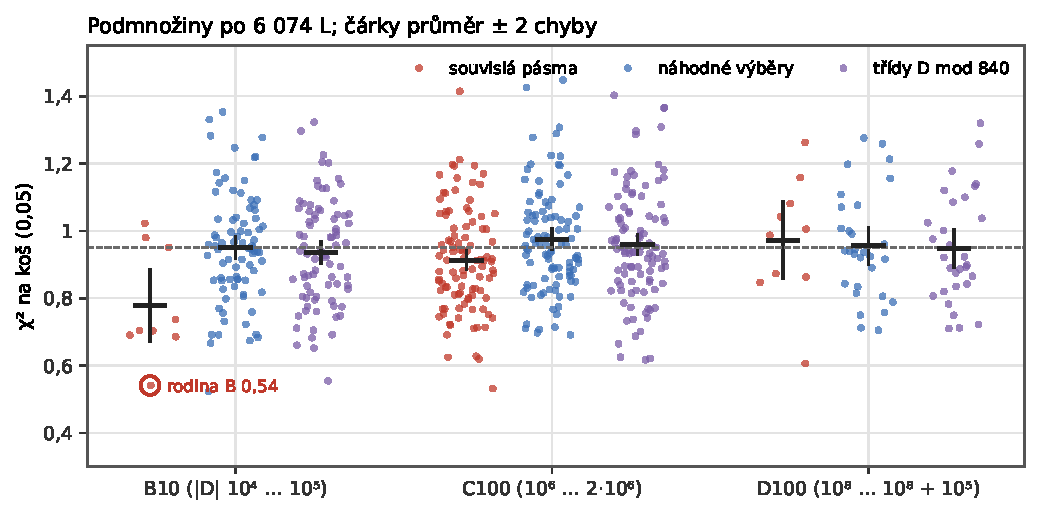
\includegraphics[width=0.95\textwidth,height=\textheight]{../../figures/04_subsets_cz.pdf}
\caption{Obrázek 4. \(\chi^2\) na koš podmnožin 6 074 L-funkcí: souvislá
pásma (červeně), náhodné výběry (modře) a náhodné výběry se třídami
\(D \bmod 840\) celé rodiny (fialově); čárky průměr \(\pm\) 2 chyby.
Kroužek označuje rodinu B, první pásmo B10.}
\end{figure}

{\small\begin{longtable}[]{@{}
  >{\raggedright\arraybackslash}p{(\columnwidth - 10\tabcolsep) * \real{0.0811}}
  >{\raggedright\arraybackslash}p{(\columnwidth - 10\tabcolsep) * \real{0.1892}}
  >{\raggedright\arraybackslash}p{(\columnwidth - 10\tabcolsep) * \real{0.1757}}
  >{\raggedright\arraybackslash}p{(\columnwidth - 10\tabcolsep) * \real{0.1757}}
  >{\raggedright\arraybackslash}p{(\columnwidth - 10\tabcolsep) * \real{0.1892}}
  >{\raggedright\arraybackslash}p{(\columnwidth - 10\tabcolsep) * \real{0.1892}}@{}}
\toprule\noalign{}
\begin{minipage}[b]{\linewidth}\raggedright
rodina
\end{minipage} & \begin{minipage}[b]{\linewidth}\raggedright
podmnožiny
\end{minipage} & \begin{minipage}[b]{\linewidth}\raggedright
\(\chi^2\)/koš 0,05
\end{minipage} & \begin{minipage}[b]{\linewidth}\raggedright
\(\chi^2\)/koš 0,1
\end{minipage} & \begin{minipage}[b]{\linewidth}\raggedright
výkon při \(k = 1 \dots 7\)
\end{minipage} & \begin{minipage}[b]{\linewidth}\raggedright
výkon při \(k = 32 \dots 79\)
\end{minipage} \\
\midrule\noalign{}
\endhead
\bottomrule\noalign{}
\endlastfoot
B10 & 9 pásem & \(0{,}779 \pm 0{,}055\) & \(0{,}686 \pm 0{,}058\) &
\(0{,}0098 \pm 0{,}0048\) & \(0{,}540 \pm 0{,}049\) \\ \addlinespace[2pt]
& 81 náhodných & \(0{,}951 \pm 0{,}018\) & \(0{,}861 \pm 0{,}023\) &
\(0{,}0433 \pm 0{,}0031\) & \(0{,}622 \pm 0{,}016\) \\ \addlinespace[2pt]
& 81 se třídami mod 840 & \(0{,}936 \pm 0{,}018\) &
\(0{,}816 \pm 0{,}020\) & \(0{,}0365 \pm 0{,}0030\) &
\(0{,}633 \pm 0{,}015\) \\ \addlinespace[2pt]
C100 & 100 pásem & \(0{,}913 \pm 0{,}015\) & \(0{,}801 \pm 0{,}020\) &
\(0{,}0187 \pm 0{,}0014\) & \(0{,}609 \pm 0{,}013\) \\ \addlinespace[2pt]
& 100 náhodných & \(0{,}976 \pm 0{,}017\) & \(0{,}930 \pm 0{,}022\) &
\(0{,}0518 \pm 0{,}0029\) & \(0{,}623 \pm 0{,}012\) \\ \addlinespace[2pt]
& 100 se třídami mod 840 & \(0{,}960 \pm 0{,}017\) &
\(0{,}897 \pm 0{,}021\) & \(0{,}0447 \pm 0{,}0027\) &
\(0{,}604 \pm 0{,}012\) \\ \addlinespace[2pt]
D100 & 10 pásem & \(0{,}973 \pm 0{,}059\) & \(0{,}888 \pm 0{,}068\) &
\(0{,}0246 \pm 0{,}0034\) & \(0{,}635 \pm 0{,}045\) \\ \addlinespace[2pt]
& 30 náhodných & \(0{,}956 \pm 0{,}029\) & \(0{,}907 \pm 0{,}040\) &
\(0{,}0517 \pm 0{,}0054\) & \(0{,}601 \pm 0{,}025\) \\ \addlinespace[2pt]
& 30 se třídami mod 840 & \(0{,}949 \pm 0{,}030\) &
\(0{,}905 \pm 0{,}034\) & \(0{,}0443 \pm 0{,}0059\) &
\(0{,}610 \pm 0{,}030\) \\ \addlinespace[2pt]
\end{longtable}}

V B10 a C100 jsou souvislá pásma pod náhodnými výběry o 3,0 a 2,8
směrodatné chyby v \(\chi^2\); v D100 se v \(\chi^2\) neliší. Kosinový
rozklad ukazuje, kde rozdíl leží (obrázek 5): na nízkých frekvencích,
\(k = 1 \dots 7\) neboli \(u < 1\), mají pásma 0,23, 0,36 a 0,48 výkonu
náhodných výběrů v B10, C100 a D100 (5,9, 10,2 a 4,3 směrodatné chyby),
na vysokých frekvencích \(k = 32 \dots 79\) žádný významný rozdíl není
(−1,6, −0,8 a +0,7). Celkové \(\chi^2\) ukáže jev jen tam, kde potlačené
nízké frekvence tvoří dost velkou část.

\begin{figure}
\centering
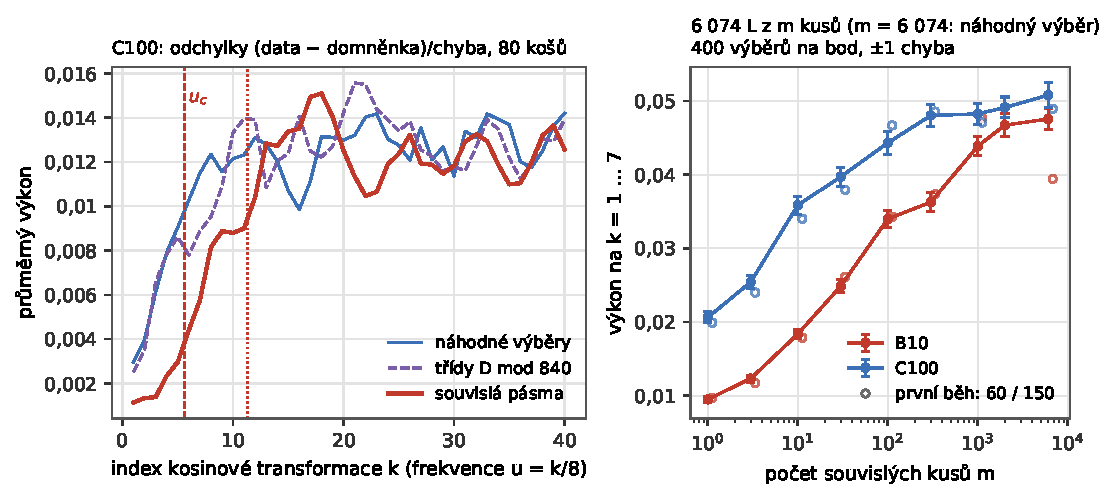
\includegraphics[width=0.95\textwidth,height=\textheight]{../../figures/05_spectrum_pieces_cz.pdf}
\caption{Obrázek 5. Vlevo: průměrný výkon kosinové transformace odchylek
v C100 pro souvislá pásma (červeně), náhodné výběry (modře) a výběry se
třídami mod 840 (fialově, čárkovaně) jako klouzavý průměr přes tři
sousední \(k\); svislé čáry \(u_c\) a \(2u_c\). Vpravo: výkon při
\(k = 1 \dots 7\) podmnožin složených z \(m\) souvislých kusů na
náhodných místech, 400 podmnožin na bod s chybou \(\pm 1\) (plně);
prázdné kroužky první běh s 60 (B10) a 150 (C100) podmnožinami na bod,
mírně posunuté doprava --- jeho zdánlivý vrchol B10 při \(m = 1\,000\)
je kolísání malého počtu náhodných podmnožin.}
\end{figure}

\textbf{Mechanismus.} Podle explicitního vzorce obsahuje odchylka
jednohladinové hustoty množiny diskriminantů \(\mathcal S\) od jejího
středu pro každé prvočíslo \(p\) člen úměrný
\(\frac{\ln p}{\sqrt p}\langle\chi_D(p)\rangle_{\mathcal S}\cos(t\ln p)\)
a od čtverců prvočísel člen s \(\langle\chi_D(p)^2\rangle_{\mathcal S}\)
a \(\cos(2t\ln p)\). V rozvinuté proměnné je
\(t\ln p = 2\pi x\,\ln p/l\) (v hlavním řádu), takže prvočíslo \(p\)
působí na frekvenci \(u = \ln p/l\). V úseku po sobě jdoucích
diskriminantů délky \(\Delta\) (v \(|D|\)) závisí \(\chi_D(p)\) na \(D\)
jen modulo \(p\) (modulo 8 pro \(p = 2\)) a pro \(p < \Delta\) prochází
průměr téměř úplné periody: je řádu \(p/N\) místo \(N^{-1/2}\) u
náhodného výběru \(N\) diskriminantů; totéž platí pro podíl \(D\)
dělitelných \(p\). Kolísání hustoty rodiny je proto potlačeno pod
\(u_c = \ln\Delta/l\) (od \(\chi_D(p)\)) a částečně až do \(2u_c\) (od
čtverců prvočísel). Pro pásma 6 074 diskriminantů je
\(\Delta \approx 10^4\) a \(u_c = 0{,}96\), 0,71 a 0,53 v B10, C100 a
D100 --- potlačené pásmo se s vodičem zužuje, jak bylo naměřeno.
Periodicita \(\chi_d(n)\) v \(d\) je standardní nástroj vět o středních
hodnotách přes diskriminanty {[}14, 15{]}. Nejbližší publikované měření
jsou murmurace kvadratických charakterů {[}16{]}: průměr
\(\chi_{8d}(p)\) přes \(d\) kolem \(X\) závisí jen na \(p/X\), pro
\(p/X \to 0\) jde k nule a mění se kolem \(p \approx X\), což autoři
spojují s přechodem jednohladinové hustoty symplektické rodiny při
nosiči 1 {[}7, 17{]}. V tomto jazyce je \(u_c = \ln\Delta/l\) tentýž
přechod pro rodinu délky \(\Delta\) místo \(X\) (náš výklad; formálněji
v oddíle 4.6). Dva testy a upozornění k náhodnému výběru:

\begin{itemize}
\tightlist
\item
  \emph{Kusy.} Podmnožina z \(m\) souvislých kusů délky \(\Delta/m\) má
  \(u_c = \ln(\Delta/m)/l\): čím kratší kusy, tím méně prvočísel uvnitř
  kusu proběhne celé periody. S 400 podmnožinami na bod roste výkon při
  \(k = 1 \dots 7\) s \(m\) z 0,0095 ± 0,0004 (\(m = 1\)) na 0,0476 ±
  0,0014 (náhodný výběr) v B10 a z 0,0206 ± 0,0008 na 0,0508 ± 0,0017 v
  C100, v mezích chyb monotónně (Spearmanova pořadová korelace s
  \(\ln m\) 1,00 v obou; obrázek 5 vpravo); nezávislé zopakování s
  jinými náhodnými místy dává totéž. B10 dosáhne náhodné hodnoty později
  než C100, protože tentýž kus má při menším vodiči vyšší mez \(u_c\)
  (\(l\) = 9,6 proti 13,1; při \(m = 300\) je \(u_c\) = 0,36 proti
  0,27), potlačení tedy sahá dál do nízkých módů. Při \(m = 1\,000\) v
  B10 nejspíš zůstává malé potlačení (0,0428 ± 0,0004 proti 0,0452 ±
  0,0012 u náhodných výběrů, průměry čtyř nezávislých běhů): kus asi
  šesti diskriminantů ještě pokryje celé periody \(p = 2, 3, 5\).
\item
  \emph{Náhodný výběr.} Každý bod je průměr přes náhodné podmnožiny a
  jeho chyba je směrodatná odchylka podmnožin dělená odmocninou jejich
  počtu. Výkon jedné podmnožiny kolísá o 60--90 \% svého průměru (je to
  součet sedmi čtverců kosinových koeficientů), takže při 60
  podmnožinách je chyba bodu asi desetina jeho hodnoty. První běh tohoto
  testu s 60 podmnožinami na bod v B10 a 150 v C100 (prázdné kroužky v
  obrázku 5) ukázal v B10 zdánlivý vrchol při \(m = 1\,000\) (0,0477 ±
  0,0046) a po něm pokles k náhodnému výběru (0,0394 ± 0,0027), o 1,5
  společné chyby mezi dvěma sousedními body. S 400 podmnožinami na bod
  vrchol zmizí (0,0439 ± 0,0013 a 0,0476 ± 0,0014) a čtyři nezávislé
  běhy po 400 podmnožinách dávají 0,0419--0,0439 při \(m = 1\,000\) a
  0,0421--0,0476 u náhodných výběrů. Krok mezi sousedními body křivky
  sestavené z náhodných výběrů je proto nálezem jen tehdy, když je velký
  proti chybám obou bodů, a náhodná hodnota B10 se uvádí jako průměr s
  chybou, ne jako jediný běh.
\item
  \emph{Zbytkové třídy.} Náhodné výběry se zastoupením celé rodiny ve
  třídách (znaménko, \(D \bmod 840\)) ustálí průměry \(\chi_D(p)\) jen
  pro \(p = 2, 3, 5, 7\); výkon na nízkých frekvencích sníží jen o
  14--16 \% (pětinu až čtvrtinu schodku pásem) a \(\chi^2\) nechají tam,
  kde jsou náhodné výběry (tabulka). Jev nese celé rozmezí prvočísel až
  po délku úseku, ne nejmenší prvočísla. Oddíl 4.4 testuje 19 modulů a
  znaménko; se čtyřikrát až pětkrát více výběry je tam snížení
  stratifikací \(D \bmod 840\) v B10 18 \% (\(z = -5{,}1\)) a v C100 a
  D100 nevýznamné.
\end{itemize}

\textbf{Rodina B.} V B10 dává devět pásem od \(|D| = 10^4\) \(\chi^2\) =
0,54, 0,69, 0,69, 0,74, 0,70, 0,98, 0,95, 1,02, 0,70; první je rodina B.
Je to nejnižší pásmo, 1,5 směrodatné odchylky pod jejich průměrem 0,78:
obecný účinek souvislosti při malém vodiči a k tomu obvyklé kolísání.
Pro celou rodinu B10 (\(\Delta = 9\cdot10^4\)) je potlačená část
vzhledem k pásu bootstrapu menší a \(\chi^2 = 0{,}87\) (pravděpodobnost
0,34). Jev je vlastnost toho, jak je rodina vybrána, ne nul jednotlivých
L-funkcí: náhodné rodiny, které pokrývají týž rozsah vodičů, ho nemají.

\hypertarget{zbytkovuxe9-tux159uxeddy-pro-19-modulux16f-a-souux10dty-charakterux16f}{%
\subsection{4.4 Zbytkové třídy pro 19 modulů a součty
charakterů}\label{zbytkovuxe9-tux159uxeddy-pro-19-modulux16f-a-souux10dty-charakterux16f}}

Oddíl 4.3 testoval jednu stratifikaci, (znaménko, \(D \bmod 840\)). Aby
se ukázalo, zda nějaký modul vytvoří jev souvislých pásem, test se
zopakoval pro 19 modulů --- prvočísla a mocniny prvočísel 3, 5, 7, 8, 9,
13, 16, 41 a 131 a složené moduly 24, 40, 120, 130, 260, 360, 369, 520,
800 a 840 --- a pro samotné znaménko \(D\) (\(M = 1\)). Všechny
podmnožiny tohoto oddílu jsou nově vylosované, nezávislé na oddílu 4.3:
první běh s 81 / 100 / 30 výběry na stratifikaci a nezávislé opakování s
jinými semínky a více výběry (300 / 300 / 100 v B10 / C100 / D100)
proběhlo pro náhodné výběry, znaménko a moduly 3, 7, 8, 16, 41, 360, 520
a 840 a prvočíslo 131 přibylo v samostatném běhu stejné velikosti.

{\small\begin{longtable}[]{@{}
  >{\raggedright\arraybackslash}p{(\columnwidth - 8\tabcolsep) * \real{0.2000}}
  >{\raggedright\arraybackslash}p{(\columnwidth - 8\tabcolsep) * \real{0.2000}}
  >{\raggedright\arraybackslash}p{(\columnwidth - 8\tabcolsep) * \real{0.2000}}
  >{\raggedright\arraybackslash}p{(\columnwidth - 8\tabcolsep) * \real{0.2000}}
  >{\raggedright\arraybackslash}p{(\columnwidth - 8\tabcolsep) * \real{0.2000}}@{}}
\toprule\noalign{}
\begin{minipage}[b]{\linewidth}\raggedright
stratifikace
\end{minipage} & \begin{minipage}[b]{\linewidth}\raggedright
\(W_{100}\) (B10 / C100 / D100)
\end{minipage} & \begin{minipage}[b]{\linewidth}\raggedright
B10
\end{minipage} & \begin{minipage}[b]{\linewidth}\raggedright
C100
\end{minipage} & \begin{minipage}[b]{\linewidth}\raggedright
D100
\end{minipage} \\
\midrule\noalign{}
\endhead
\bottomrule\noalign{}
\endlastfoot
náhodné & 1 / 1 / 1 & 0,0440 & 0,0489 & 0,0499 \\ \addlinespace[2pt]
souvislá pásma & 0,04 / 0,04 / 0,05 & 0,0098 (\(-7{,}0\)) & 0,0187
(\(-16{,}2\)) & 0,0246 (\(-6{,}4\)) \\ \addlinespace[2pt]
jen znaménko & 1,00 / 1,00 / 1,00 & 0,0452 (\(+0{,}6\)) & 0,0490
(\(+0{,}0\)) & 0,0497 (\(-0{,}0\)) \\ \addlinespace[2pt]
\(D \bmod 3\) & 0,96 / 0,96 / 0,96 & 0,0468 (\(+1{,}5\)) & 0,0508
(\(+0{,}9\)) & 0,0480 (\(-0{,}6\)) \\ \addlinespace[2pt]
\(D \bmod 5\) & 0,95 / 0,95 / 0,95 & 0,0479 (\(+1{,}0\)) & 0,0510
(\(+0{,}6\)) & 0,0573 (\(+1{,}3\)) \\ \addlinespace[2pt]
\(D \bmod 7\) & 0,94 / 0,94 / 0,94 & 0,0436 (\(-0{,}2\)) & 0,0508
(\(+0{,}9\)) & 0,0487 (\(-0{,}3\)) \\ \addlinespace[2pt]
\(D \bmod 8\) & 0,98 / 0,98 / 0,98 & 0,0414 (\(-1{,}5\)) & 0,0480
(\(-0{,}5\)) & 0,0457 (\(-1{,}4\)) \\ \addlinespace[2pt]
\(D \bmod 9\) & 0,96 / 0,96 / 0,96 & 0,0424 (\(-0{,}5\)) & 0,0493
(\(+0{,}1\)) & 0,0552 (\(+0{,}9\)) \\ \addlinespace[2pt]
\(D \bmod 13\) & 0,94 / 0,94 / 0,94 & 0,0442 (\(+0{,}1\)) & 0,0485
(\(-0{,}1\)) & 0,0512 (\(+0{,}2\)) \\ \addlinespace[2pt]
\(D \bmod 16\) & 0,98 / 0,98 / 0,98 & 0,0425 (\(-0{,}9\)) & 0,0518
(\(+1{,}4\)) & 0,0478 (\(-0{,}6\)) \\ \addlinespace[2pt]
\(D \bmod 24\) & 0,94 / 0,94 / 0,94 & 0,0431 (\(-0{,}3\)) & 0,0503
(\(+0{,}4\)) & 0,0425 (\(-1{,}4\)) \\ \addlinespace[2pt]
\(D \bmod 40\) & 0,93 / 0,93 / 0,93 & 0,0390 (\(-1{,}7\)) & 0,0464
(\(-0{,}7\)) & 0,0422 (\(-1{,}4\)) \\ \addlinespace[2pt]
\(D \bmod 41\) & 0,96 / 0,96 / 0,96 & 0,0445 (\(+0{,}3\)) & 0,0505
(\(+0{,}8\)) & 0,0438 (\(-2{,}0\)) \\ \addlinespace[2pt]
\(D \bmod 120\) & 0,89 / 0,89 / 0,89 & 0,0420 (\(-0{,}7\)) & 0,0506
(\(+0{,}5\)) & 0,0555 (\(+0{,}9\)) \\ \addlinespace[2pt]
\(D \bmod 130\) & 0,89 / 0,89 / 0,89 & 0,0460 (\(+0{,}6\)) & 0,0531
(\(+1{,}4\)) & 0,0508 (\(+0{,}2\)) \\ \addlinespace[2pt]
\(D \bmod 131\) & 1,00 / 1,00 / 1,00 & 0,0451 (\(+0{,}6\)) & 0,0505
(\(+0{,}7\)) & 0,0547 (\(+1{,}2\)) \\ \addlinespace[2pt]
\(D \bmod 260\) & 0,89 / 0,89 / 0,89 & 0,0447 (\(+0{,}2\)) & 0,0526
(\(+1{,}0\)) & 0,0485 (\(-0{,}2\)) \\ \addlinespace[2pt]
\(D \bmod 360\) & 0,90 / 0,89 / 0,89 & 0,0402 (\(-2{,}1\)) & 0,0468
(\(-1{,}1\)) & 0,0456 (\(-1{,}3\)) \\ \addlinespace[2pt]
\(D \bmod 369\) & 0,93 / 0,92 / 0,93 & 0,0434 (\(-0{,}2\)) & 0,0551
(\(+1{,}7\)) & 0,0511 (\(+0{,}3\)) \\ \addlinespace[2pt]
\(D \bmod 520\) & 0,88 / 0,87 / 0,88 & 0,0425 (\(-0{,}8\)) & 0,0476
(\(-0{,}7\)) & 0,0479 (\(-0{,}6\)) \\ \addlinespace[2pt]
\(D \bmod 800\) & 0,94 / 0,93 / 0,94 & 0,0415 (\(-0{,}8\)) & 0,0479
(\(-0{,}3\)) & 0,0395 (\(-2{,}4\)) \\ \addlinespace[2pt]
\(D \bmod 840\) & 0,84 / 0,83 / 0,84 & 0,0359 (\(-5{,}1\)) & 0,0462
(\(-1{,}4\)) & 0,0518 (\(+0{,}6\)) \\ \addlinespace[2pt]
\end{longtable}}

Výkon kosinových koeficientů \(k = 1 \dots 7\) podmnožin 6 074 L-funkcí,
průměr přes 81--681 (B10), 100--700 (C100) a 30--230 (D100) výběrů
(všechny běhy dohromady; souvislých pásem 9 / 100 / 10), v závorce \(z\)
= (stratifikace − náhodné) / společná chyba. \(W_{100}\) je přesný zbylý
podíl stratifikovaného výběru bez vracení (oddíl 3), pro všechny
stratifikace.

V C100 a D100 se žádná stratifikace od náhodných výběrů neliší víc, než
dá 40 testů náhodou: za 2 směrodatné chyby jsou jen D100 mod 800
(\(z = -2{,}4\), 30 výběrů) a mod 41 (\(-2{,}0\)). V B10 je jediné
zřetelné snížení \(D \bmod 840\) (\(z = -5{,}1\)), za ním 360
(\(-2{,}1\)). Vyrovnání \(D \bmod 8\) nebo \(D \bmod 16\), které ustálí
\(\chi_D(2)\), nerozhoduje (\(z = -1{,}5 / -0{,}5 / -1{,}4\) a
\(-0{,}9 / +1{,}4 / -0{,}6\)) a samotné znaménko nedělá nic. První běh s
30 výběry dal pro D100 mod 840 \(0{,}0606 \pm 0{,}0073\); s opakováním
(130 výběrů) je hodnota \(0{,}0518 \pm 0{,}0028\), jako u náhodných
výběrů.

\textbf{Součty charakterů bez nul.} Náhodné výběry mají rozptyl průměrů
\(\chi_D(p)\) výběru z konečného souboru do 0,4 \% (medián poměru 1,0011
/ 1,0022 / 0,9960 z 300 losování). Pro stratifikaci podle \(M\) je
přesný rozptyl stratifikovaného výběru bez vracení u prvočísel dělících
\(M\) nejvýš 0,07 náhodné hodnoty (pro \(p = 2\) jen při \(8 \mid M\);
zbytek je zaokrouhlení počtů ve třídách) a u každého jiného prvočísla
1,000--1,014. Podíl \(W_{100}\), který stratifikovaná podmnožina
zachová, je proto u všech 20 stratifikací aspoň 0,83 (u 840 0,84 / 0,83
/ 0,84; tabulka), proti 0,04--0,05 u souvislých pásem. Přímka dvěma body
každé rodiny --- náhodnými výběry (\(W = 1\)) a souvislými pásmy ---
dává pro všech 60 stratifikovaných podmnožin \(\chi^2 = 82{,}05\) s
kovariancí obou společných bodů (\(p = 0{,}03\); střední 95\% rozmezí
pro 60 stupňů volnosti je 40,5--83,3) a pro 33 bodů první verze tohoto
oddílu \(\chi^2 = 47{,}7\) (\(p = 0{,}05\)). Směr souhlasí: žádná
stratifikace se k pásmům ani nepřiblíží (obrázek 6 vlevo). Velikost
souhlasí jen na hraně: 42 z 60 odchylek je kladných (průměr
\(z = +0{,}56\)), stratifikace sníží výkon nul na nízkých frekvencích o
něco méně, než přímka předpoví. Pravděpodobný důvod je, že přímka přičte
celý schodek pásem prvočíslům do 100, kdežto pásma potlačí i prvočísla
mezi 100 a \(10^4\) (profil níže), kterých se modul nedotkne. Dvě
kontroly: strmost proložená samotnými 20 stratifikacemi, dělená strmostí
přímky, dává podíl schodku pásem, který nesou \(p \le 100\), 1,09 ±
0,26, 0,53 ± 0,26 a 0,02 ± 0,54 v B10, C100 a D100 (spojeně 0,72 ± 0,17)
--- klesá s vodičem, protože nízké módy nesou stále větší prvočísla, ale
jen na úrovni 1,5--2 chyb; a stejné váhy \((\ln p)^2/p\) přes všechna
prvočísla nízkých módů (\(W_E\), pásma 0,18 / 0,53 / 0,75) posun
odstraní (průměr \(z = +0{,}02\)), ale v B10 přestřelí
(\(\chi^2 = 91{,}0\), \(p = 0{,}006\), B10 mod 840 4,1 chyby pod
předpovědí). Obě osy pocházejí z různých dat --- na jedné nuly, na druhé
hodnoty charakterů --- takže souhlas ve směru je nezávislá kontrola
mechanismu oddílu 4.3: modul ustálí jen prvočísla, která ho dělí, kdežto
nízké frekvence nesou všechna prvočísla až do tisíců; jak se rozptyl
\(\chi_D(p)\) převádí na výkon na nízkých frekvencích, je pochopeno ve
směru, ne ve velikosti.

\begin{figure}
\centering
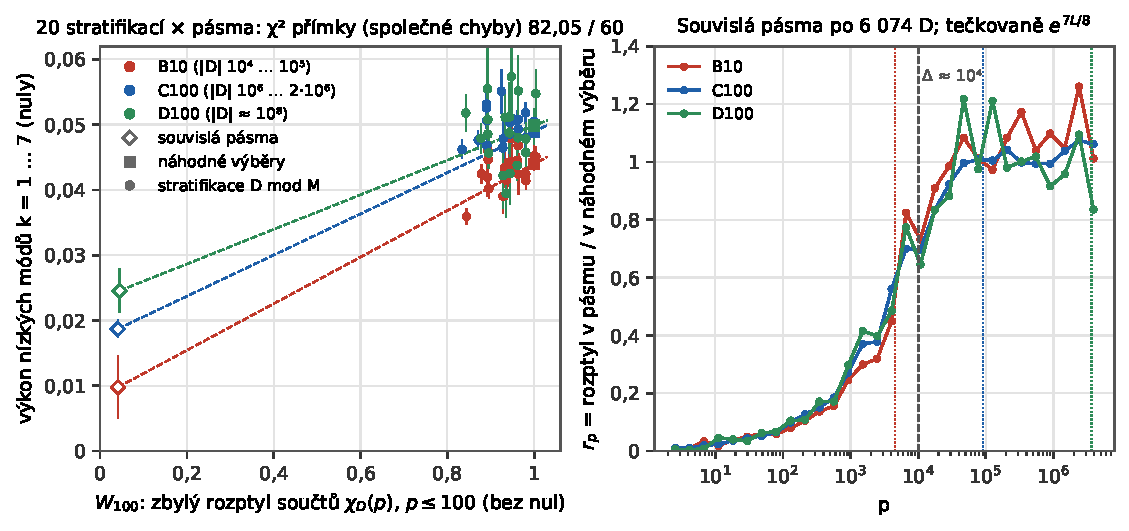
\includegraphics[width=0.95\textwidth,height=\textheight]{../../figures/06_moduli_characters_cz.pdf}
\caption{Obrázek 6. Vlevo: přesný zbylý podíl \(W_{100}\) váženého
rozptylu průměrů \(\chi_D(p)\), \(p \le 100\) (z charakterů, bez nul),
proti výkonu nul na nízkých frekvencích \(k = 1 \dots 7\) (z nul, bez
charakterů) pro náhodné výběry (čtverce), 20 stratifikací (body) a
souvislá pásma (kosočtverce) rodin B10, C100 a D100, s chybou \(\pm 1\);
čárkovaně přímka dvěma body každé rodiny. Vpravo: profil \(r_p\)
souvislých pásem 6 074 diskriminantů (582 prvočísel do \(4\cdot10^6\) v
logaritmických koších); čárkovaně šířka pásma \(\Delta \approx 10^4\),
tečkovaně \(e^{7L/8}\) pro každou rodinu.}
\end{figure}

\textbf{Závislost na vodiči.} Profil \(r_p\) souvislých pásem je ve
třech rodinách, jejichž pásma mají všechna šířku \(\Delta \approx 10^4\)
v \(|D|\), táž funkce \(p\): 0,04--0,05 pro \(p \le 100\), 0,12--0,17 do
\(10^3\), 0,29--0,41 do \(10^4\), 0,84--0,90 do \(10^5\) a nad tím asi 1
(obrázek 6 vpravo). Mód \(k\) nesou prvočísla s \(\ln p \approx kL/8\),
\(L = \ln(|D|/\pi)\), tedy až do \(e^{7L/8} \approx 4\cdot10^3\),
\(9\cdot10^4\) a \(4\cdot10^6\) v B10, C100 a D100; podíl vážený \(k\),
\(W_k = \sum_k k\,r(e^{kL/8})/28\), roste
\(0{,}22 \to 0{,}61 \to 0{,}70\), kdežto naměřený poměr výkonu pásem a
náhodných výběrů na nízkých frekvencích roste
\(0{,}22 \pm 0{,}11 \to 0{,}38 \pm 0{,}03 \to 0{,}49 \pm 0{,}07\).
Pořadí i směr souhlasí, velikost pro C100 ne (7 chyb). Převod rozptylu
\(\chi_D(p)\) na výkon souvislých pásem na nízkých frekvencích je tedy
pochopen ve směru, ne ve velikosti.

\hypertarget{prvnuxed-nula}{%
\subsection{4.5 První nula}\label{prvnuxed-nula}}

\begin{figure}
\centering
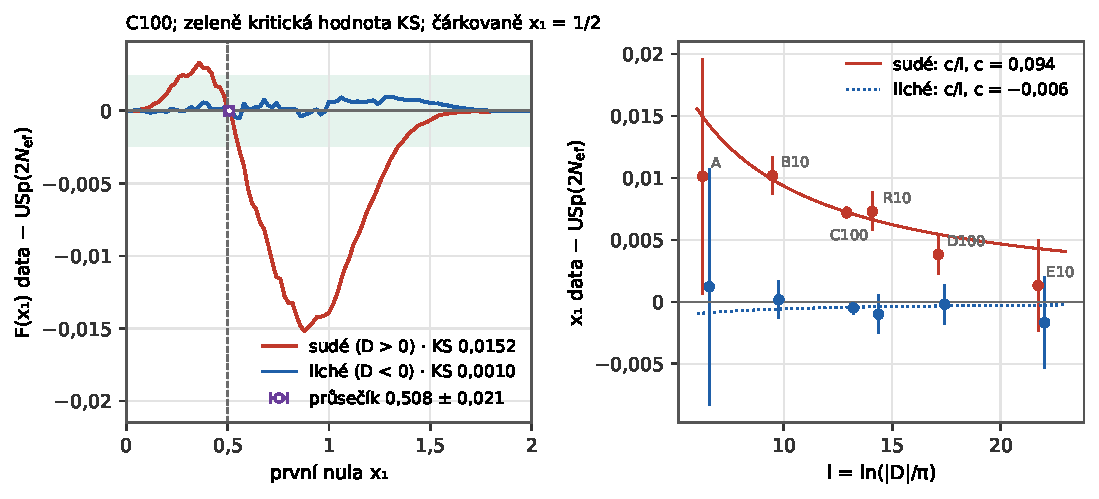
\includegraphics[width=0.95\textwidth,height=\textheight]{../../figures/07_first_zero_cz.pdf}
\caption{Obrázek 7. Vlevo: distribuční funkce první nuly v C100 minus
USp\((2N_{\mathrm{ef}})\) pro sudé (červeně) a liché (modře) charaktery;
zeleně kritická hodnota Kolmogorovova--Smirnovova testu, čárkovaně
\(x_1 = \frac12\) (konec intervalu, na kterém se určuje
\(N_{\mathrm{ef}}\)), fialově průsečík sudé křivky s nulou s chybou
(mřížka 0,001, bootstrap). Vpravo: odchylka průměrné první nuly od
USp\((2N_{\mathrm{ef}})\) podle \(l = \ln(|D|/\pi)\) v šesti
nepřekrývajících se rodinách, s proklady \(c/l\).}
\end{figure}

USp\((2N)\) s \(N = \frac12\ln(|D|/\pi)\) první nulu nepopíše: její
průměr je 0,67--0,75 proti naměřeným 0,58--0,70 a
Kolmogorovova--Smirnovova vzdálenost je 0,06--0,14, 1,6× až 53× kritické
hodnoty. Efektivní \(N_{\mathrm{ef}}\) určené domněnkou poměrů je
1,5--4,5, dvakrát až třikrát menší než \(\frac12 l\), a
USp\((2N_{\mathrm{ef}})\) dává průměrnou první nulu ve všech rodinách do
1,1 \%. Rozdělení podle znaménka s chybami C100, B10, D100, E10 a R10
ukáže rozdíl (obrázek 7):

{\small\begin{longtable}[]{@{}
  >{\raggedright\arraybackslash}p{(\columnwidth - 10\tabcolsep) * \real{0.0822}}
  >{\raggedleft\arraybackslash}p{(\columnwidth - 10\tabcolsep) * \real{0.0959}}
  >{\raggedright\arraybackslash}p{(\columnwidth - 10\tabcolsep) * \real{0.2466}}
  >{\raggedright\arraybackslash}p{(\columnwidth - 10\tabcolsep) * \real{0.1644}}
  >{\raggedright\arraybackslash}p{(\columnwidth - 10\tabcolsep) * \real{0.2466}}
  >{\raggedright\arraybackslash}p{(\columnwidth - 10\tabcolsep) * \real{0.1644}}@{}}
\toprule\noalign{}
\begin{minipage}[b]{\linewidth}\raggedright
rodina
\end{minipage} & \begin{minipage}[b]{\linewidth}\raggedleft
\(l\)
\end{minipage} & \begin{minipage}[b]{\linewidth}\raggedright
sudé (\(D > 0\)): \(x_1 - x_1^{\mathrm{ef}}\)
\end{minipage} & \begin{minipage}[b]{\linewidth}\raggedright
KS / kritická
\end{minipage} & \begin{minipage}[b]{\linewidth}\raggedright
liché (\(D < 0\)): \(x_1 - x_1^{\mathrm{ef}}\)
\end{minipage} & \begin{minipage}[b]{\linewidth}\raggedright
KS / kritická
\end{minipage} \\
\midrule\noalign{}
\endhead
\bottomrule\noalign{}
\endlastfoot
A & 6,41 & \(+0{,}0101 \pm 0{,}0095\) & 0,032 / 0,055 &
\(+0{,}0012 \pm 0{,}0096\) & 0,017 / 0,055 \\ \addlinespace[2pt]
B10 & 9,62 & \(+0{,}0102 \pm 0{,}0015\) & 0,025 / 0,008 &
\(+0{,}0002 \pm 0{,}0015\) & 0,003 / 0,008 \\ \addlinespace[2pt]
C100 & 13,06 & \(+0{,}0072 \pm 0{,}0005\) & 0,015 / 0,0025 &
\(-0{,}0005 \pm 0{,}0005\) & 0,0010 / 0,0025 \\ \addlinespace[2pt]
R10 & 14,23 & \(+0{,}0073 \pm 0{,}0016\) & 0,014 / 0,008 &
\(-0{,}0010 \pm 0{,}0016\) & 0,003 / 0,008 \\ \addlinespace[2pt]
D100 & 17,28 & \(+0{,}0038 \pm 0{,}0016\) & 0,008 / 0,008 &
\(-0{,}0002 \pm 0{,}0016\) & 0,003 / 0,008 \\ \addlinespace[2pt]
E10 & 21,88 & \(+0{,}0013 \pm 0{,}0037\) & 0,006 / 0,017 &
\(-0{,}0017 \pm 0{,}0037\) & 0,006 / 0,018 \\ \addlinespace[2pt]
\end{longtable}}

Pro liché charaktery dává USp\((2N_{\mathrm{ef}})\) celé rozdělení první
nuly v mezích chyb při každém vodiči od \(10^3\) do \(10^{10}\) (v C100
je Kolmogorovova--Smirnovova vzdálenost 0,0010 při kritické hodnotě
0,0025); proklad \(c/l\) dává \(c = -0{,}006 \pm 0{,}006\). Pro sudé
charaktery leží první nula výš: o 14,8 směrodatné chyby v C100, 6,6 v
B10, 4,6 v R10. Odchylka s vodičem klesá a proloží se \(c/l\) s
\(c = 0{,}094 \pm 0{,}006\) (\(\chi^2 = 2{,}1\) při 5 stupních
volnosti); stálý posun dává \(\chi^2 = 10{,}7\) a \(c/l^2\) 7,6.
Proložení na rodinách s \(l < 15\) předpoví pro D100 0,0055 a pro E10
0,0043, naměřeno \(0{,}0038 \pm 0{,}0016\) a \(0{,}0013 \pm 0{,}0037\).
Jeden efektivní parametr tedy na obě znaménka nestačí; sudé charaktery
potřebují opravu nižšího řádu, kterou současná data měří, ale
neodvozují.

\textbf{Kde sudá křivka protíná nulu.} Na mřížce 0,001 místo 0,02 mění
rozdíl \(F(x_1) - \mathrm{USp}(2N_{\mathrm{ef}})\) sudých charakterů
C100 znaménko v \(x_1 = 0{,}508 \pm 0{,}021\) (bootstrap přes L-funkce,
400 opakování; obrázek 7 vlevo); sudá a lichá křivka se protnou v
\(0{,}504 \pm 0{,}034\) a v B10 leží průsečík v \(0{,}488 \pm 0{,}038\).
Čisté posunutí USp\((2N_{\mathrm{ef}})\) o naměřený rozdíl průměru
(0,0072) ani změna měřítka se stejným průměrem průsečík nedají ---
rozdíl má pak všude jedno znaménko. Poloha průsečíku ale pochází z
kalibrace, ne z nul. \(N_{\mathrm{ef}}\) se volí tak, aby
USp\((2N_{\mathrm{ef}})\) měla v \([0, \frac12]\) hustotu domněnky
poměrů, tedy tam i stejný očekávaný počet nul (oddíl 3), a data ji mají
také (sudé charaktery C100: 0,6303 proti 0,6303). Protože pro počet
\(N(a)\) nul v \([0, a]\) platí
\(P(x_1 \le a) = E[N(a)] - \sum_{k \ge 2} P(N(a) \ge k)\), obě
distribuční funkce se pak v \(a\) téměř shodnou, až na členy dvou a více
nul v \([0, a]\). Určí-li se \(N_{\mathrm{ef}}\) místo toho na
\([0, a]\), průsečík se posouvá s \(a\):

{\small\begin{longtable}[]{@{}
  >{\raggedright\arraybackslash}p{(\columnwidth - 12\tabcolsep) * \real{0.3143}}
  >{\raggedleft\arraybackslash}p{(\columnwidth - 12\tabcolsep) * \real{0.1143}}
  >{\raggedleft\arraybackslash}p{(\columnwidth - 12\tabcolsep) * \real{0.1143}}
  >{\raggedleft\arraybackslash}p{(\columnwidth - 12\tabcolsep) * \real{0.1143}}
  >{\raggedleft\arraybackslash}p{(\columnwidth - 12\tabcolsep) * \real{0.1143}}
  >{\raggedleft\arraybackslash}p{(\columnwidth - 12\tabcolsep) * \real{0.1143}}
  >{\raggedleft\arraybackslash}p{(\columnwidth - 12\tabcolsep) * \real{0.1143}}@{}}
\toprule\noalign{}
\begin{minipage}[b]{\linewidth}\raggedright
interval kalibrace \([0, a]\)
\end{minipage} & \begin{minipage}[b]{\linewidth}\raggedleft
\(a = 0{,}3\)
\end{minipage} & \begin{minipage}[b]{\linewidth}\raggedleft
0,4
\end{minipage} & \begin{minipage}[b]{\linewidth}\raggedleft
0,5
\end{minipage} & \begin{minipage}[b]{\linewidth}\raggedleft
0,6
\end{minipage} & \begin{minipage}[b]{\linewidth}\raggedleft
0,7
\end{minipage} & \begin{minipage}[b]{\linewidth}\raggedleft
sklon
\end{minipage} \\
\midrule\noalign{}
\endhead
\bottomrule\noalign{}
\endlastfoot
C100: \(N_{\mathrm{ef}}\) & 2,278 & 2,352 & 2,432 & 2,517 & 2,612 & \\ \addlinespace[2pt]
C100: průsečík & 0,291 & 0,416 & 0,508 & 0,595 & 0,767 & 1,13 \\ \addlinespace[2pt]
B10: \(N_{\mathrm{ef}}\) & 1,641 & 1,751 & 1,854 & 1,950 & 2,052 & \\ \addlinespace[2pt]
B10: průsečík & 0,289 & 0,414 & 0,488 & 0,598 & 0,771 & 1,15 \\ \addlinespace[2pt]
\end{longtable}}

Ve všech případech leží průsečík nejvýš 0,071 od \(a\). Že průsečík leží
v \(\frac12\), je proto jako vlastnost první nuly zamítnuto: označuje
konec intervalu kalibrace. S kalibrací v \(\frac12\) zůstává tvar: sudé
charaktery mají víc prvních nul pod \(\frac12\) (vrchol \(+0{,}0034\) v
0,36) a méně mezi \(\frac12\) a asi 1,3 (minimum \(-0{,}0152\) v
\(0{,}874 \pm 0{,}018\)), což posunutí ani změna měřítka nevytvoří. V A,
R10, D100 a E10 je kladná část v šumu a průsečík se určit nedá
(0,30--0,36 ± 0,09--0,11). Druhý průsečík v C100 není: křivka se vrátí
do pásma Kolmogorovova--Smirnovova testu v \(1{,}341 \pm 0{,}009\) (B10:
\(1{,}183 \pm 0{,}017\), návrat tedy závisí na vodiči a není to
\(\frac32\)), v 1,5 je ještě \(-0{,}00063 \pm 0{,}00007\) a s nulou
splyne až u konce modelu, \(0{,}98\,N_{\mathrm{ef}} = 2{,}38\).

\hypertarget{pux159esnuxe1-oux10dekuxe1vuxe1nuxed-vrstvy-vyvuxe1ux17eenuxe9-vuxfdbux11bry-a-vazba-muxf3dux16f}{%
\subsection{4.6 Přesná očekávání, vrstvy, vyvážené výběry a vazba
módů}\label{pux159esnuxe1-oux10dekuxe1vuxe1nuxed-vrstvy-vyvuxe1ux17eenuxe9-vuxfdbux11bry-a-vazba-muxf3dux16f}}

S chybou každého koše z očekávaného počtu předpovědi rodiny (Pearsonův
tvar, jako studie II) je \(c_k\) podmnožiny \(\mathcal S\) o \(N\)
L-funkcích průměrem pevných čísel \(y_{ik}\) přes \(\mathcal S\),
jednoho na L-funkci, a jeho očekávaný čtverec přes všechny podmnožiny
daného způsobu výběru je \(\bar y_k^2\) plus rozptyl průměru:
\(S_k^2/N\,(1 - N/n)\) pro náhodný výběr, totéž přes
\(\lfloor n/\ell\rfloor\) kusů pro kusy \(\ell\) po sobě jdoucích
diskriminantů, \(\sum_c k_c(1 - k_c/n_c)S_{ck}^2/N^2\) pro stratifikaci
a přesný průměr přes všech \(n - N + 1\) začátků pro jeden úsek. Tato
vrstva 0 nepotřebuje žádná náhodná čísla. Statistika testu (chyba z
pozorovaného počtu, oddíly 4.3--4.4) se od ní liší jen málo; ten rozdíl
se losuje na týchž podmnožinách (vrstva 1, 200 podmnožin) a zpřesní tam,
kde zbyla největší chyba (vrstva 2, nejvýš 1 600 podmnožin, cílová chyba
\(2\cdot10^{-4}\)). Rozdíl kolísá třikrát až pětkrát méně než statistika
sama a chyba každého bodu klesne 3,6 / 3,8 / 4,1× (B10 / C100 / D100)
proti losování samotné statistiky; všechny návrhy používají tatáž
náhodná čísla.

{\small\begin{longtable}[]{@{}
  >{\raggedright\arraybackslash}p{(\columnwidth - 12\tabcolsep) * \real{0.1250}}
  >{\raggedleft\arraybackslash}p{(\columnwidth - 12\tabcolsep) * \real{0.1458}}
  >{\raggedleft\arraybackslash}p{(\columnwidth - 12\tabcolsep) * \real{0.1458}}
  >{\raggedleft\arraybackslash}p{(\columnwidth - 12\tabcolsep) * \real{0.1458}}
  >{\raggedleft\arraybackslash}p{(\columnwidth - 12\tabcolsep) * \real{0.1458}}
  >{\raggedleft\arraybackslash}p{(\columnwidth - 12\tabcolsep) * \real{0.1458}}
  >{\raggedleft\arraybackslash}p{(\columnwidth - 12\tabcolsep) * \real{0.1458}}@{}}
\toprule\noalign{}
\begin{minipage}[b]{\linewidth}\raggedright
návrh
\end{minipage} & \begin{minipage}[b]{\linewidth}\raggedleft
B10 vrstva 0
\end{minipage} & \begin{minipage}[b]{\linewidth}\raggedleft
B10 odhad
\end{minipage} & \begin{minipage}[b]{\linewidth}\raggedleft
C100 vrstva 0
\end{minipage} & \begin{minipage}[b]{\linewidth}\raggedleft
C100 odhad
\end{minipage} & \begin{minipage}[b]{\linewidth}\raggedleft
D100 vrstva 0
\end{minipage} & \begin{minipage}[b]{\linewidth}\raggedleft
D100 odhad
\end{minipage} \\
\midrule\noalign{}
\endhead
\bottomrule\noalign{}
\endlastfoot
náhodný výběr (\(\ell = 1\)) & 0,0443 & \(0{,}0455 \pm 0{,}0002\) &
0,0488 & \(0{,}0506 \pm 0{,}0002\) & 0,0479 &
\(0{,}0488 \pm 0{,}0002\) \\ \addlinespace[2pt]
trojice (\(\ell = 3\)) & 0,0432 & \(0{,}0443 \pm 0{,}0002\) & 0,0480 &
\(0{,}0493 \pm 0{,}0002\) & 0,0474 & \(0{,}0485 \pm 0{,}0002\) \\ \addlinespace[2pt]
\(\ell = 10\) & 0,0408 & \(0{,}0420 \pm 0{,}0002\) & 0,0468 &
\(0{,}0485 \pm 0{,}0002\) & 0,0470 & \(0{,}0480 \pm 0{,}0002\) \\ \addlinespace[2pt]
\(\ell = 100\) & 0,0289 & \(0{,}0300 \pm 0{,}0002\) & 0,0405 &
\(0{,}0418 \pm 0{,}0002\) & 0,0424 & \(0{,}0432 \pm 0{,}0002\) \\ \addlinespace[2pt]
\(\ell = 1\,000\) & 0,0134 & \(0{,}0143 \pm 0{,}0002\) & 0,0286 &
\(0{,}0299 \pm 0{,}0002\) & 0,0346 & \(0{,}0352 \pm 0{,}0002\) \\ \addlinespace[2pt]
třídy \(D \bmod 840\) & 0,0369 & \(0{,}0377 \pm 0{,}0002\) & 0,0456 &
\(0{,}0464 \pm 0{,}0002\) & 0,0469 & \(0{,}0476 \pm 0{,}0002\) \\ \addlinespace[2pt]
jeden úsek (všechny začátky) & 0,0079 & 0,0093 & 0,0185 & 0,0200 &
0,0292 & 0,0295 \\ \addlinespace[2pt]
\end{longtable}}

\begin{figure}
\centering
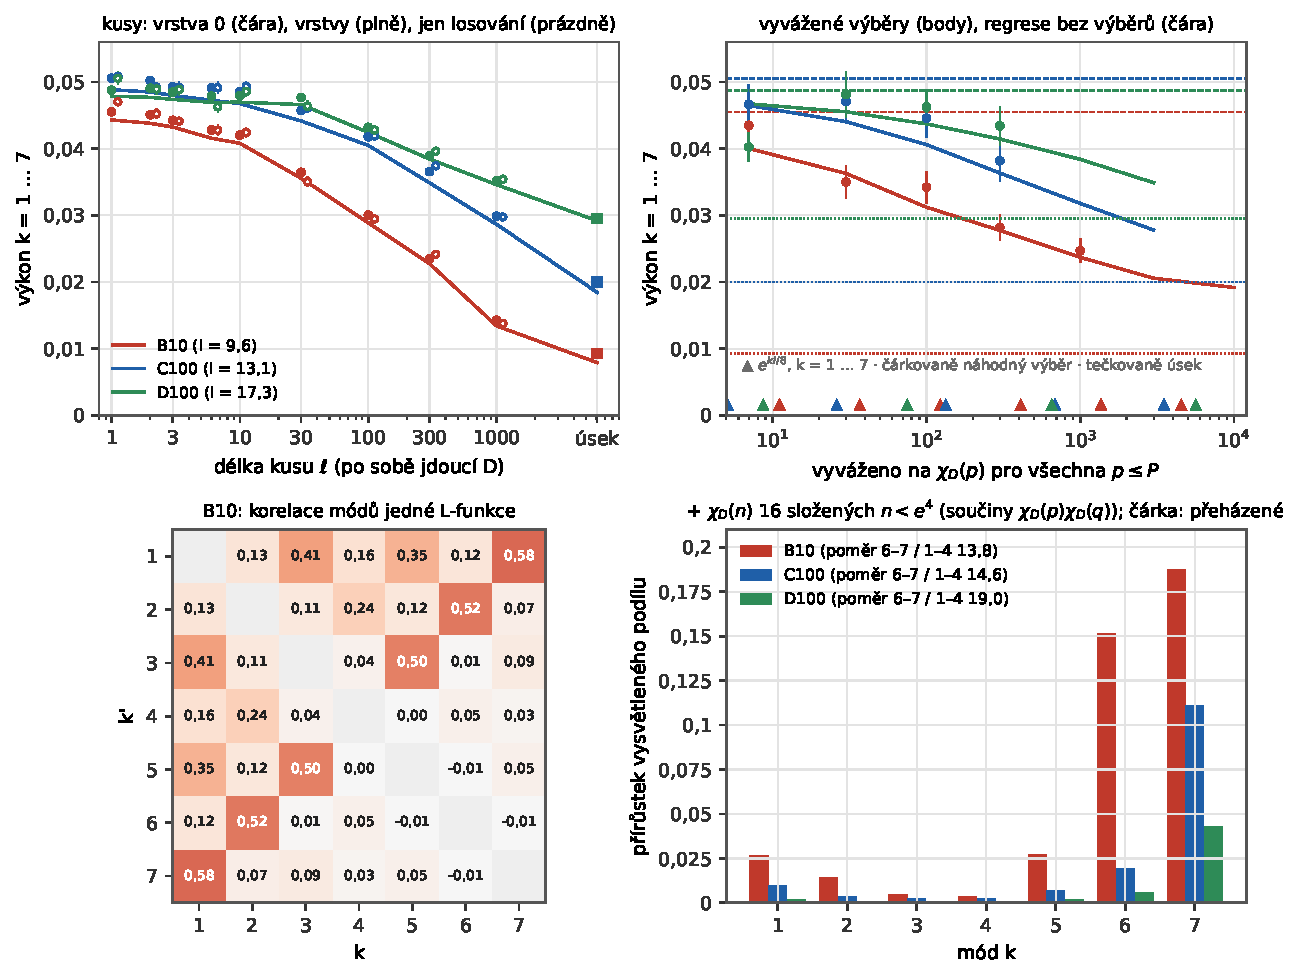
\includegraphics[width=0.95\textwidth,height=\textheight]{../../figures/08_layers_cz.pdf}
\caption{Obrázek 8. Vlevo nahoře: výkon nízkých frekvencí podmnožin 6
074 L-funkcí z náhodně rozmístěných kusů \(\ell\) po sobě jdoucích
diskriminantů (čára vrstva 0 bez losování, plně vrstvový odhad ±1 chyba,
prázdně jen losování, vpravo jeden úsek). Vpravo nahoře: výběry vyvážené
na \(\chi_D(p)\) pro \(p \le P\) (body ±1 chyba) a vrstva 0 z regrese
(čára); trojúhelníky \(e^{kl/8}\). Vlevo dole: korelace příspěvků jedné
L-funkce mezi módy v B10. Vpravo dole: přírůstek vysvětleného podílu
rozptylu každého módu po přidání \(\chi_D(n)\) 16 složených \(n < e^4\),
čárky nulový model.}
\end{figure}

\textbf{Kusy a trojice.} Výkon klesá s délkou kusu. Už trojice po sobě
jdoucích diskriminantů leží pod náhodným výběrem: 0,972 náhodné hodnoty
v B10 (4,7 chyby) a 0,975 v C100 (4,3), jak předpoví vrstva 0 (0,976 a
0,983); v D100 je pokles (0,995) pod rozlišením, protože při větším
vodiči nesou nízké módy větší prvočísla, která tři sousedé nevyrovnají.

\textbf{Posun o několik procent.} Statistika testu leží nad vrstvou 0 o
\(0{,}0012 \pm 0{,}0002 / 0{,}0017 \pm 0{,}0002 / 0{,}0009 \pm 0{,}0002\)
u náhodného výběru (2,7 / 3,5 / 1,9 \%) a rozdíl je kladný u všech 30
návrhů; náhodný šum by měl obě znaménka. Jde o zkreslení odhadu:
podmnožina 6 074 L-funkcí má v nejnižším koši jen 3,4 / 2,8 / 2,5
očekávaných nul a ve druhém asi 20 (\(x < 0{,}1\)), kde je dělení
odmocninou pozorovaného počtu silně nelineární. S chybou z očekávaného
počtu jen v těchto dvou koších zmizí v B10 84 \% posunu; s Pearsonovým
tvarem všude se losovaná statistika rovná vrstvě 0 do
\((1{,}5 \pm 1{,}5)\cdot10^{-6}\). Delta metoda druhého řádu ho
nezachytí, tři nebo čtyři nuly jsou mimo obor její platnosti. Dřívější
dojem asi 5 \% byl tento posun spolu s chybou losování.

\textbf{Vyvážené výběry.} Náhodný výběr lze držet ve složení celé rodiny
v \(\chi_D(p)\) a \(\chi_D(p)^2\) pro všechna prvočísla \(p \le P\)
(náhodný začátek a výměny, které zmenší nevyváženost s vahou
\((\ln p)^2/p\); 100 výběrů na \(P\)). Jeho vrstva 0 plyne z regrese
\(y_{ik}\) na tyto charaktery: vyvážení ponechá jen zbytkový rozptyl. V
B10 je změřený výkon \(0{,}0435 \pm 0{,}0029\),
\(0{,}0350 \pm 0{,}0025\), \(0{,}0342 \pm 0{,}0024\),
\(0{,}0282 \pm 0{,}0019\), \(0{,}0247 \pm 0{,}0018\) pro \(P\) = 7, 30,
100, 300, 1~000 a lineární statistika týchž výběrů souhlasí s regresí ve
všech 13 případech tří rodin do tří chyb (nejvíc D100, \(P = 7\): 3,0).
Mód \(k\) se vyrovná, když \(P\) dosáhne \(\ln p \approx k\,l/8\): v B10
(\(l = 9{,}6\)) mód 1 prvočísly do 7, mód 4 do 100 a mód 6 do 1 000. S
\(P = 10^4\) je vrstva 0 v B10 0,0192, stále nad úsekem (0,0079); zbytek
nesou větší prvočísla a složená \(n\).

\textbf{Vazba módů a intermodulace.} Příspěvky jedné L-funkce k módům
\(k\) a \(8 - k\) jsou korelované: 1--7 / 2--6 / 3--5 B10 0,58 / 0,52 /
0,50 · C100 0,47 / 0,42 / 0,40 · D100 0,39 / 0,35 / 0,35, kdežto nuly
jako Poissonův proces dávají přesně 0 (s Pearsonovým tvarem je jejich
kovariance \(N\)-násobek jednotkové matice). Mód 8 je střední rozestup
nul a \(k\) a \(8 - k\) jsou jeho postranní pásma. Vazba je druhého řádu
v charakterech: když se k regresi na všechna \(p \le 300\) přidají
\(\chi_D(n)\) 16 bezčtvercových složených \(n < e^4\) (součiny
\(\chi_D(p)\chi_D(q)\) prvočísel do 23, u 30 a 42 tří), vzroste
vysvětlený podíl módu 7 o 0,188 / 0,111 / 0,043 a módu 6 o 0,152 / 0,019
/ 0,006, módů 1--4 nejvýš o 0,026; tytéž příznaky přeházené mezi
L-funkcemi dají nejvýš 0,0003. Malá prvočísla nesou mód 1 (v B10 i 2),
jejich součiny zrcadlový mód --- intermodulace s nosnou středního
rozestupu. Vyvážení na \(\chi_D(n)\) všech \(n \le 1\,000\) sníží vrstvu
0 na 0,0162 / 0,0253 / 0,0352 proti 0,0237 / 0,0318 / 0,0384 jen s
prvočísly; jeden úsek, který vyrovná všechna \(n\) pod svou šířkou, má
0,0079 / 0,0185 / 0,0292.

\textbf{Filtry ve frekvenci prvočísel.} Pro jednu L-funkci a sudou
testovací funkci \(\phi\) s kompaktním nosičem \(\hat\phi\) vstupuje v
explicitním vzorci prvočíslo \(p\) s vahou \(\ln p/\sqrt p\) na
frekvenci \(u_p = \ln p/l\) (člen \(\chi_D(p)\hat\phi(u_p)\)) a jeho
čtverec na \(2u_p\); v kosinových módech je to \(k_p = 8u_p\).
Podmnožina kolísá jen přes průměry
\(\langle\chi_D(n)\rangle_{\mathcal S}\). Pro celou rodinu do \(X\) je
průměr \(\chi_D(p)\) přes \(D\) zanedbatelný pro \(p\) hluboko pod \(X\)
(celé periody) a pro \(p \gtrsim X\) ne; odtud pochází přechod u
\(|u| = 1\) ve Fourierově transformaci hustoty USp i v podmínce nosiče
\(|u| < 1\) Rubinsteinovy věty {[}7{]} (za GRH, pro \(n\)-hladinové
hustoty \(\sum|u_j| < 1\); rozšíření do 2 Gao {[}20{]} a
Levinson--Miller {[}21{]}; členy nižšího řádu pro rozšířený nosič
{[}17{]}). Úsek šířky \(\Delta\) u \(|D|\) má tutéž vlastnost jen pro
\(n \lesssim \Delta\): průměr prochází celé periody a neúplný zbytek
omezuje nerovnost Pólyi--Vinogradova,
\(|\sum_{d \in I}(d/p)| < \sqrt p\ln p\) pro každý interval \(I\), takže
pro \(p\ln^2 p \ll \Delta\) je průměr hluboko pod \(\Delta^{-1/2}\)
náhodného výběru. (U základních diskriminantů podmínka bezčtvercovosti
přesnou periodicitu porušuje; jde proto o heuristiku, ne o větu.) Úsek
je tedy dolní propust ve frekvenci prvočísel do \(u_c = \ln\Delta/l\)
--- obdoba nosiče 1, v níž \(X\) nahradí \(\Delta\); pro
\(\Delta = |D|\) je \(u_c = 1\). V módech je \(k_c = 8u_c\) = 7,66 /
5,64 / 4,26 (B10 / C100 / D100) a poměr vrstvy 0 jednoho úseku a
náhodného výběru je pod \(k_c\) 0,10--0,28 / 0,20--0,43 / 0,34--0,44 a
nad \(k_c\) --- / 0,44--0,54 / 0,61--0,93 (průměr nad / pod 1,61 v C100
a 1,97 v D100). Přechod je pozvolný, protože profil \(r_p\) roste s
\(p/\Delta\) plynule (oddíl 4.4).

Stratifikace podle \(M\) je hřebenový filtr. Pevné složení (znaménko,
\(D \bmod 840\)) zafixuje průměry každé funkce těchto zbytků: čáry
\(\chi_D(p)\) a \(\chi_D(p)^2\) pro \(p\) = 2, 3, 5, 7 na \(k_p\) =
0,58, 0,91, 1,34, 1,62 v B10 (0,42--1,19 v C100, 0,32--0,90 v D100),
znaménko a všechny součiny \(\chi_D(n)\), \(n \mid 210\) --- čáry
intermodulace. Vrstva 0 se bez losování rozloží (regrese na tyto
příznaky, nakonec všech 840 obsazených tříd): náhodný výběr → čáry → +
znaménko → + součiny → + součiny a čáry krát znaménko → třídy = B10
0,0443 → 0,0400 → 0,0400 → 0,0375 → 0,0374 → 0,0362; C100 0,0488 →
0,0465 → 0,0465 → 0,0456 → 0,0456 → 0,0450; D100 0,0479 → 0,0467 →
0,0467 → 0,0464 → 0,0464 → 0,0456 (celočíselné zastoupení návrhu dává
0,0369 / 0,0456 / 0,0469). Čáry nesou 53 / 62 / 50 \% snížení, součiny
33 / 24 / 17 \%, zbytek struktury tříd 14 / 14 / 33 \% a znaménko nic.
Proto D mod 840 působí v B10 (oddíl 4.4, \(z = -5{,}1\)) a při větších
vodičích málo: čáry 2, 3, 5, 7 tam leží pod módem 1.

\hypertarget{pux159epoux10det-po-hladinuxe1ch-stejnuxe1-pravidla-jinuxfd-princip}{%
\subsection{4.7 Přepočet po hladinách: stejná pravidla, jiný
princip}\label{pux159epoux10det-po-hladinuxe1ch-stejnuxe1-pravidla-jinuxfd-princip}}

Oddíly 4.1--4.6 zůstávají tak, jak byly spočteny. Tento oddíl je
rozšíření: každé číslo oddílů 4.3--4.5, které vzniklo z náhodných
podmnožin, je přepočteno principem oddílu 4.6 --- vrstva 0 bez losování,
losuje se jen malý rozdíl skutečného testu --- a se stejnými pravidly:
stejné návrhy (náhodné výběry, znaménko a 19 modulů se stejným
přidělením největším zbytkem, \(m\) kusů na stejné mřížce bloků), stejná
velikost 6 074 L-funkcí a stejná statistika s chybou z pozorovaného
počtu. U kusů plyne přesná vrstva 0 podmíněním na dva bloky pořadí \(r\)
a \(r + 1\) (\(r\) delších kusů a zbytek jsou pak dva nezávislé prosté
výběry bloků), celková pravděpodobnost je 1 s přesností \(10^{-12}\).
Každý návrh má 200 výběrů a další až do 1 800, dokud chyba výkonu
nízkých frekvencí nespadne pod \(2\cdot10^{-4}\); výběr \(r\) všech
návrhů používá týž generátor (společná náhodná čísla). Pevná pásma,
jeden kus (\(m = 1\)) a jeden úsek přes všech \(n - N + 1\) začátků
losování vůbec nepotřebují. Kontrola vrstvy 0 v týchž výběrech (losovaná
Pearsonova statistika proti vrstvě 0) dává pro 84 návrhů a čtyři
statistiky střední \(z^2\) 1,13 a \(|z| \le 3{,}0\). Chyba výkonu
nízkých frekvencí je 1,6--4,6× menší než se samotným losováním (medián
3,7; nejméně u 3 a 10 kusů v B10), chyba vysokých módů a \(\chi^2\) na
koš 4--10×.

{\small\begin{longtable}[]{@{}
  >{\raggedright\arraybackslash}p{(\columnwidth - 12\tabcolsep) * \real{0.1429}}
  >{\raggedright\arraybackslash}p{(\columnwidth - 12\tabcolsep) * \real{0.1429}}
  >{\raggedright\arraybackslash}p{(\columnwidth - 12\tabcolsep) * \real{0.1429}}
  >{\raggedright\arraybackslash}p{(\columnwidth - 12\tabcolsep) * \real{0.1429}}
  >{\raggedright\arraybackslash}p{(\columnwidth - 12\tabcolsep) * \real{0.1429}}
  >{\raggedright\arraybackslash}p{(\columnwidth - 12\tabcolsep) * \real{0.1429}}
  >{\raggedright\arraybackslash}p{(\columnwidth - 12\tabcolsep) * \real{0.1429}}@{}}
\toprule\noalign{}
\begin{minipage}[b]{\linewidth}\raggedright
stratifikace
\end{minipage} & \begin{minipage}[b]{\linewidth}\raggedright
B10 původně
\end{minipage} & \begin{minipage}[b]{\linewidth}\raggedright
B10 po hladinách
\end{minipage} & \begin{minipage}[b]{\linewidth}\raggedright
C100 původně
\end{minipage} & \begin{minipage}[b]{\linewidth}\raggedright
C100 po hladinách
\end{minipage} & \begin{minipage}[b]{\linewidth}\raggedright
D100 původně
\end{minipage} & \begin{minipage}[b]{\linewidth}\raggedright
D100 po hladinách
\end{minipage} \\
\midrule\noalign{}
\endhead
\bottomrule\noalign{}
\endlastfoot
náhodné & 0,0440 & \(0{,}0456 \pm 0{,}0002\) & 0,0489 &
\(0{,}0512 \pm 0{,}0003\) & 0,0499 & \(0{,}0487 \pm 0{,}0002\) \\ \addlinespace[2pt]
jen znaménko & 0,0452 (\(+0{,}6\)) & 0,0457 (\(+0{,}1\)) & 0,0490
(\(+0{,}0\)) & 0,0508 (\(-1{,}0\)) & 0,0497 (\(-0{,}0\)) & 0,0487
(\(-0{,}1\)) \\ \addlinespace[2pt]
\(D \bmod 3\) & 0,0468 (\(+1{,}5\)) & 0,0444 (\(-4{,}4\)) & 0,0508
(\(+0{,}9\)) & 0,0495 (\(-4{,}5\)) & 0,0480 (\(-0{,}6\)) & 0,0487
(\(-0{,}2\)) \\ \addlinespace[2pt]
\(D \bmod 5\) & 0,0479 (\(+1{,}0\)) & 0,0445 (\(-4{,}0\)) & 0,0510
(\(+0{,}6\)) & 0,0501 (\(-3{,}0\)) & 0,0573 (\(+1{,}3\)) & 0,0487
(\(-0{,}2\)) \\ \addlinespace[2pt]
\(D \bmod 7\) & 0,0436 (\(-0{,}2\)) & 0,0445 (\(-3{,}7\)) & 0,0508
(\(+0{,}9\)) & 0,0499 (\(-3{,}6\)) & 0,0487 (\(-0{,}3\)) & 0,0489
(\(+0{,}8\)) \\ \addlinespace[2pt]
\(D \bmod 8\) & 0,0414 (\(-1{,}5\)) & 0,0439 (\(-5{,}3\)) & 0,0480
(\(-0{,}5\)) & 0,0499 (\(-3{,}7\)) & 0,0457 (\(-1{,}4\)) & 0,0483
(\(-1{,}6\)) \\ \addlinespace[2pt]
\(D \bmod 9\) & 0,0424 (\(-0{,}5\)) & 0,0449 (\(-2{,}7\)) & 0,0493
(\(+0{,}1\)) & 0,0503 (\(-2{,}4\)) & 0,0552 (\(+0{,}9\)) & 0,0486
(\(-0{,}7\)) \\ \addlinespace[2pt]
\(D \bmod 13\) & 0,0442 (\(+0{,}1\)) & 0,0450 (\(-2{,}1\)) & 0,0485
(\(-0{,}1\)) & 0,0500 (\(-3{,}3\)) & 0,0512 (\(+0{,}2\)) & 0,0483
(\(-1{,}2\)) \\ \addlinespace[2pt]
\(D \bmod 16\) & 0,0425 (\(-0{,}9\)) & 0,0443 (\(-4{,}5\)) & 0,0518
(\(+1{,}4\)) & 0,0501 (\(-3{,}0\)) & 0,0478 (\(-0{,}6\)) & 0,0485
(\(-0{,}9\)) \\ \addlinespace[2pt]
\(D \bmod 24\) & 0,0431 (\(-0{,}3\)) & 0,0428 (\(-9{,}1\)) & 0,0503
(\(+0{,}4\)) & 0,0492 (\(-5{,}7\)) & 0,0425 (\(-1{,}4\)) & 0,0481
(\(-2{,}1\)) \\ \addlinespace[2pt]
\(D \bmod 40\) & 0,0390 (\(-1{,}7\)) & 0,0419 (\(-12{,}8\)) & 0,0464
(\(-0{,}7\)) & 0,0493 (\(-5{,}3\)) & 0,0422 (\(-1{,}4\)) & 0,0483
(\(-1{,}4\)) \\ \addlinespace[2pt]
\(D \bmod 41\) & 0,0445 (\(+0{,}3\)) & 0,0455 (\(-0{,}5\)) & 0,0505
(\(+0{,}8\)) & 0,0502 (\(-2{,}8\)) & 0,0438 (\(-2{,}0\)) & 0,0490
(\(+1{,}1\)) \\ \addlinespace[2pt]
\(D \bmod 120\) & 0,0420 (\(-0{,}7\)) & 0,0405 (\(-17{,}3\)) & 0,0506
(\(+0{,}5\)) & 0,0480 (\(-8{,}4\)) & 0,0555 (\(+0{,}9\)) & 0,0477
(\(-4{,}2\)) \\ \addlinespace[2pt]
\(D \bmod 130\) & 0,0460 (\(+0{,}6\)) & 0,0438 (\(-6{,}4\)) & 0,0531
(\(+1{,}4\)) & 0,0497 (\(-4{,}0\)) & 0,0508 (\(+0{,}2\)) & 0,0479
(\(-2{,}8\)) \\ \addlinespace[2pt]
\(D \bmod 131\) & 0,0451 (\(+0{,}6\)) & 0,0457 (\(+0{,}1\)) & 0,0505
(\(+0{,}7\)) & 0,0503 (\(-2{,}6\)) & 0,0547 (\(+1{,}2\)) & 0,0488
(\(+0{,}2\)) \\ \addlinespace[2pt]
\(D \bmod 260\) & 0,0447 (\(+0{,}2\)) & 0,0438 (\(-6{,}1\)) & 0,0526
(\(+1{,}0\)) & 0,0494 (\(-5{,}1\)) & 0,0485 (\(-0{,}2\)) & 0,0482
(\(-1{,}9\)) \\ \addlinespace[2pt]
\(D \bmod 360\) & 0,0402 (\(-2{,}1\)) & 0,0405 (\(-17{,}8\)) & 0,0468
(\(-1{,}1\)) & 0,0481 (\(-8{,}9\)) & 0,0456 (\(-1{,}3\)) & 0,0477
(\(-4{,}0\)) \\ \addlinespace[2pt]
\(D \bmod 369\) & 0,0434 (\(-0{,}2\)) & 0,0443 (\(-4{,}6\)) & 0,0551
(\(+1{,}7\)) & 0,0497 (\(-4{,}4\)) & 0,0511 (\(+0{,}3\)) & 0,0489
(\(+0{,}5\)) \\ \addlinespace[2pt]
\(D \bmod 520\) & 0,0425 (\(-0{,}8\)) & 0,0419 (\(-12{,}7\)) & 0,0476
(\(-0{,}7\)) & 0,0483 (\(-7{,}9\)) & 0,0479 (\(-0{,}6\)) & 0,0478
(\(-3{,}2\)) \\ \addlinespace[2pt]
\(D \bmod 800\) & 0,0415 (\(-0{,}8\)) & 0,0428 (\(-8{,}8\)) & 0,0479
(\(-0{,}3\)) & 0,0489 (\(-6{,}5\)) & 0,0395 (\(-2{,}4\)) & 0,0480
(\(-2{,}1\)) \\ \addlinespace[2pt]
\(D \bmod 840\) & 0,0359 (\(-5{,}1\)) & 0,0378 (\(-26{,}6\)) & 0,0462
(\(-1{,}4\)) & 0,0464 (\(-13{,}5\)) & 0,0518 (\(+0{,}6\)) & 0,0479
(\(-2{,}9\)) \\ \addlinespace[2pt]
souvislá pásma & 0,0098 & 0,0098 (\(-7{,}5\)) & 0,0187 & 0,0187
(\(-23{,}0\)) & 0,0246 & 0,0246 (\(-7{,}1\)) \\ \addlinespace[2pt]
jeden úsek, všechny začátky & --- & 0,0093 & --- & 0,0200 & --- &
0,0295 \\ \addlinespace[2pt]
\end{longtable}}

Oddíl 4.4 po hladinách: výkon kosinových koeficientů \(k = 1 \dots 7\)
podmnožin 6 074 L-funkcí, původně (tabulka oddílu 4.4, 81--700 výběrů) a
po hladinách (vrstva 0 přesně a 200--1 800 výběrů rozdílu; chyba
0,0002--0,0003 u každé stratifikace), v závorce \(z\) proti náhodným
výběrům téhož sloupce. Souvislá pásma a úsek přes všechny začátky jsou
přesné; \(z\) pásem používá rozptyl 9 / 100 / 10 pásem.

\textbf{Zbytkové třídy.} S přesnými hodnotami snižují výkon nízkých
frekvencí stratifikace ve všech třech rodinách. Vrstva 0, přesná a bez
chyby, je nižší než u náhodných výběrů pro každý modul (o
0,00002--0,0074 v B10, 0,0001--0,0033 v C100 a 0,00005--0,0013 v D100) a
odhady po hladinách leží víc než 3 chyby pod náhodnými výběry u 15, 16 a
3 z 19 modulů v B10, C100 a D100 (\(D \bmod 840\): \(z = -26{,}6\),
\(-13{,}5\), \(-2{,}9\); \(D \bmod 120\) a 360 v D100 \(-4{,}2\) a
\(-4{,}0\)). Nejmenší účinek mají znaménko, 41 a 131, stratifikace s
\(W_{100} \ge 0{,}96\) (vrstva 0 nižší nejvýš o 0,0004); v C100 je
jejich \(z\) \(-1{,}0\), \(-2{,}8\) a \(-2{,}6\) víc, než vysvětlí
jejich přesný rozdíl vrstvy 0 (nejvýš 0,0003), a pochází z losované
části obou sloupců, takže dva moduly C100 blízko \(-3\) (\(D \bmod 5\) a
16, \(-3{,}02\) a \(-3{,}04\)) jsou započteny s touto výhradou. Věta
oddílu 4.4, že v C100 a D100 se žádná stratifikace neliší nad náhodu,
byla mez rozlišení 30--700 výběrů. Velikost závěr oddílu 4.4 drží:
\(D \bmod 840\) odebere 17 / 9,5 / 1,6 \% náhodné hodnoty, souvislá
pásma 79 / 64 / 50 \%, takže nízké \(\chi^2\) nezpůsobuje rovnováha
zbytkových tříd.

{\small\begin{longtable}[]{@{}
  >{\raggedright\arraybackslash}p{(\columnwidth - 16\tabcolsep) * \real{0.1111}}
  >{\raggedright\arraybackslash}p{(\columnwidth - 16\tabcolsep) * \real{0.1111}}
  >{\raggedright\arraybackslash}p{(\columnwidth - 16\tabcolsep) * \real{0.1111}}
  >{\raggedright\arraybackslash}p{(\columnwidth - 16\tabcolsep) * \real{0.1111}}
  >{\raggedright\arraybackslash}p{(\columnwidth - 16\tabcolsep) * \real{0.1111}}
  >{\raggedright\arraybackslash}p{(\columnwidth - 16\tabcolsep) * \real{0.1111}}
  >{\raggedright\arraybackslash}p{(\columnwidth - 16\tabcolsep) * \real{0.1111}}
  >{\raggedright\arraybackslash}p{(\columnwidth - 16\tabcolsep) * \real{0.1111}}
  >{\raggedright\arraybackslash}p{(\columnwidth - 16\tabcolsep) * \real{0.1111}}@{}}
\toprule\noalign{}
\begin{minipage}[b]{\linewidth}\raggedright
kusy \(m\)
\end{minipage} & \begin{minipage}[b]{\linewidth}\raggedright
B10 opakování
\end{minipage} & \begin{minipage}[b]{\linewidth}\raggedright
B10 po hladinách
\end{minipage} & \begin{minipage}[b]{\linewidth}\raggedright
B10 vrstva 0
\end{minipage} & \begin{minipage}[b]{\linewidth}\raggedright
C100 opakování
\end{minipage} & \begin{minipage}[b]{\linewidth}\raggedright
C100 po hladinách
\end{minipage} & \begin{minipage}[b]{\linewidth}\raggedright
C100 vrstva 0
\end{minipage} & \begin{minipage}[b]{\linewidth}\raggedright
D100 po hladinách
\end{minipage} & \begin{minipage}[b]{\linewidth}\raggedright
D100 vrstva 0
\end{minipage} \\
\midrule\noalign{}
\endhead
\bottomrule\noalign{}
\endlastfoot
1 & \(0{,}0095 \pm 0{,}0004\) & 0,0093\(^{*}\) & 0,0079 &
\(0{,}0206 \pm 0{,}0008\) & 0,0200\(^{*}\) & 0,0185 & 0,0295\(^{*}\) &
0,0292 \\ \addlinespace[2pt]
3 & \(0{,}0123 \pm 0{,}0005\) & \(0{,}0129 \pm 0{,}0002\) & 0,0117 &
\(0{,}0254 \pm 0{,}0009\) & \(0{,}0248 \pm 0{,}0002\) & 0,0232 &
\(0{,}0334 \pm 0{,}0002\) & 0,0324 \\ \addlinespace[2pt]
10 & \(0{,}0184 \pm 0{,}0007\) & \(0{,}0183 \pm 0{,}0002\) & 0,0176 &
\(0{,}0359 \pm 0{,}0012\) & \(0{,}0340 \pm 0{,}0002\) & 0,0322 &
\(0{,}0409 \pm 0{,}0002\) & 0,0401 \\ \addlinespace[2pt]
30 & \(0{,}0249 \pm 0{,}0009\) & \(0{,}0248 \pm 0{,}0002\) & 0,0238 &
\(0{,}0397 \pm 0{,}0013\) & \(0{,}0387 \pm 0{,}0002\) & 0,0371 &
\(0{,}0405 \pm 0{,}0002\) & 0,0397 \\ \addlinespace[2pt]
100 & \(0{,}0340 \pm 0{,}0011\) & \(0{,}0331 \pm 0{,}0002\) & 0,0321 &
\(0{,}0443 \pm 0{,}0016\) & \(0{,}0438 \pm 0{,}0002\) & 0,0420 &
\(0{,}0443 \pm 0{,}0002\) & 0,0433 \\ \addlinespace[2pt]
300 & \(0{,}0363 \pm 0{,}0013\) & \(0{,}0392 \pm 0{,}0002\) & 0,0377 &
\(0{,}0480 \pm 0{,}0015\) & \(0{,}0471 \pm 0{,}0002\) & 0,0452 &
\(0{,}0482 \pm 0{,}0002\) & 0,0475 \\ \addlinespace[2pt]
1000 & \(0{,}0439 \pm 0{,}0013\) & \(0{,}0428 \pm 0{,}0002\) & 0,0415 &
\(0{,}0483 \pm 0{,}0014\) & \(0{,}0489 \pm 0{,}0002\) & 0,0472 &
\(0{,}0507 \pm 0{,}0002\) & 0,0504 \\ \addlinespace[2pt]
2000 & \(0{,}0467 \pm 0{,}0016\) & \(0{,}0489 \pm 0{,}0002\) & 0,0473 &
\(0{,}0491 \pm 0{,}0014\) & \(0{,}0497 \pm 0{,}0002\) & 0,0480 &
\(0{,}0473 \pm 0{,}0002\) & 0,0454 \\ \addlinespace[2pt]
\end{longtable}}

Oddíl 4.3 po hladinách: podmnožiny z \(m\) kusů po sobě jdoucích
diskriminantů (náhodné polohy na mřížce bloků), původně (opakování se
400 podmnožinami, oddíl 4.3) a po hladinách, s přesnou vrstvou 0.
\(^{*}\) \(m = 1\): průměr přes všech \(n - N\) začátků, bez losování.

\textbf{Kusy.} Hodnoty po hladinách souhlasí s opakováním oddílu 4.3 v
rámci společné chyby (nejvíc B10 \(m = 300\): 2,3 chyby), s chybou
2,5--7× menší (6--7× pro \(m \ge 100\)). Vrstva 0 se přesně rozloží na
člen průměru (čtverec středního příspěvku návrhu) a člen rozptylu. V B10
a C100 roste člen rozptylu s \(m\) monotónně k náhodné hodnotě, jak
vyžaduje postupná ztráta efektu; v D100, kde je podmnožina desetina
rodiny, téměř (poklesy o 0,0004 u \(m = 30\) a 0,0006 u \(m = 2\,000\)).
Body nad náhodnou hodnotou, B10 \(m = 2\,000\)
(\(0{,}0489 \pm 0{,}0002\) proti \(0{,}0456 \pm 0{,}0002\)) a D100
\(m = 1\,000\) (\(0{,}0507\) proti \(0{,}0487\)), nese člen průměru ---
\(0{,}0059\) proti \(0{,}0002\) u náhodných výběrů v B10, \(0{,}0071\)
proti \(0{,}0029\) v D100 ---, což je vlastnost návrhu: s kusy po třech
na blocích po čtyřech bere podmnožina tři ze čtyř po sobě jdoucích
diskriminantů a složení rodiny v tomto pořadí není složení náhodného
výběru.

\textbf{Přímka dvěma body.} S původními hodnotami dávala přímka mezi
náhodnými výběry (\(W = 1\)) a souvislými pásmy pro 60 stratifikovaných
podmnožin \(\chi^2 = 82{,}05\) (\(p = 0{,}03\)). S přesnými hodnotami
dává \(\chi^2 = 841{,}8\) pro 60 s pásmy a \(1\,110{,}5\) s úsekem přes
všechny začátky jako druhým bodem (\(p < 10^{-130}\)), 42--43 z 60
odchylek kladných a střední \(z\) \(+1{,}6\) / \(+1{,}8\). Bez
jakéhokoli losování je snížení vrstvy 0 stratifikacemi v průměru 0,89 /
0,56 / 0,39 snížení, které dává přímka, v B10 / C100 / D100 (obrázek 9
vpravo nahoře). \(W_{100}\) určuje směr, ne velikost, a velikost s
vodičem klesá. Totéž platí pro závislost pásem na vodiči: přesný poměr
úseku přes všechny začátky a náhodných výběrů je 0,204 / 0,391 / 0,606
(původně \(0{,}22 \pm 0{,}11\), \(0{,}38 \pm 0{,}03\),
\(0{,}49 \pm 0{,}07\)) proti \(W_k\) = 0,22 / 0,61 / 0,70 --- B10
souhlasí, C100 a D100 leží níž.

\textbf{Explicitní formule a duální člen.} Pro jednu L-funkci dává
explicitní formule počet nul přesně; část závislá na charakteru má u
prvočísla \(p\) diagonální členy \(n = p^k\), tedy koeficient
\(-\frac{1}{\pi}\ln p \sum_k p^{-k/2} I(k\ln p)\) přes lichá \(k\) u
\(\chi_D(p)\) a přes sudá \(k\) u \(\chi_D(p)^2\), kde \(I(w)\) je
integrál \(\cos(wt)\) přes koš. Promítnuté do kosinových módů \(y_{ik}\)
oddílu 4.6 se tyto váhy dají bez fitu porovnat s regresí \(y_{ik}\) na
\(\chi_D(p)\) a \(\chi_D(p)^2\) pro \(p \le 100\) (175 koeficientů na
rodinu). Popíší směr, ne velikost: sklon je 0,52--0,60 a v oknech \(x\)
pod 4 leží fitovaná váha \(\chi_D(2)\) až 51 chyb od diagonální hodnoty
(B10, \(x\) = 2,5--4). Chybějící část pochází z členu domněnky poměrů,
který dává sinus ve \(W_{\mathrm{USp}}\) (duální člen). Pro podrodinu s
\(\chi_D(p) = e\) je místní faktor u \(p\) v obou členech
\((1 - e\,p^{-1/2-\gamma})/(1 - e\,p^{-1/2-\alpha})\) místo průměru
rodiny: diagonální člen vrátí váhy výše a duální člen se změní faktorem
\(A_e/A_p\) místních faktorů v \(\alpha = -it\), \(\gamma = it\). S
přidanými duálními vahami je sklon 0,995--0,999 ve třech rodinách a
0,94--1,01 po módech (největší odchylka B10 \(k = 4\):
\(0{,}978 \pm 0{,}004\)):

{\small\begin{longtable}[]{@{}
  >{\raggedright\arraybackslash}p{(\columnwidth - 14\tabcolsep) * \real{0.1250}}
  >{\raggedright\arraybackslash}p{(\columnwidth - 14\tabcolsep) * \real{0.1250}}
  >{\raggedright\arraybackslash}p{(\columnwidth - 14\tabcolsep) * \real{0.1250}}
  >{\raggedright\arraybackslash}p{(\columnwidth - 14\tabcolsep) * \real{0.1250}}
  >{\raggedright\arraybackslash}p{(\columnwidth - 14\tabcolsep) * \real{0.1250}}
  >{\raggedright\arraybackslash}p{(\columnwidth - 14\tabcolsep) * \real{0.1250}}
  >{\raggedright\arraybackslash}p{(\columnwidth - 14\tabcolsep) * \real{0.1250}}
  >{\raggedright\arraybackslash}p{(\columnwidth - 14\tabcolsep) * \real{0.1250}}@{}}
\toprule\noalign{}
\begin{minipage}[b]{\linewidth}\raggedright
rodina
\end{minipage} & \begin{minipage}[b]{\linewidth}\raggedright
sklon, diagonální
\end{minipage} & \begin{minipage}[b]{\linewidth}\raggedright
sklon, s duálním členem
\end{minipage} & \begin{minipage}[b]{\linewidth}\raggedright
okna \(\chi^2\) (30 koef.), diagonální → duální
\end{minipage} & \begin{minipage}[b]{\linewidth}\raggedright
vysvětlený podíl \(k = 1 \dots 4\), diagonální → duální
\end{minipage} & \begin{minipage}[b]{\linewidth}\raggedright
mod 8: přesně / duální / diagonální
\end{minipage} & \begin{minipage}[b]{\linewidth}\raggedright
mod 840: přesně / duální / diagonální
\end{minipage} & \begin{minipage}[b]{\linewidth}\raggedright
úsek: přesně / duální / diagonální
\end{minipage} \\
\midrule\noalign{}
\endhead
\bottomrule\noalign{}
\endlastfoot
B10 & \(0{,}5227 \pm 0{,}0011\) & \(0{,}9948 \pm 0{,}0018\) & 6469 → 5,4
& \(-0{,}53\) / \(-0{,}05\) / 0,33 / 0,55 → 0,56 / 0,69 / 0,76 / 0,80 &
0,00131 / 0,00130 / 0,00197 & 0,00737 / 0,00462 / 0,00995 & 0,0364 /
0,0325 / 0,0871 \\ \addlinespace[2pt]
C100 & \(0{,}5780 \pm 0{,}0004\) & \(0{,}9993 \pm 0{,}0007\) & 33797 →
9,2 & \(-0{,}32\) / 0,12 / 0,40 / 0,52 → 0,55 / 0,71 / 0,78 / 0,76 &
0,00074 / 0,00074 / 0,00121 & 0,00328 / 0,00178 / 0,00358 & 0,0304 /
0,0230 / 0,0651 \\ \addlinespace[2pt]
D100 & \(0{,}5980 \pm 0{,}0019\) & \(0{,}9993 \pm 0{,}0029\) & 1746 →
27,8 & 0,08 / 0,36 / 0,47 / \(-0{,}07\) → 0,54 / 0,68 / 0,68 / 0,10 &
0,00032 / 0,00033 / 0,00060 & 0,00095 / 0,00099 / 0,00224 & 0,0187 /
0,0122 / 0,0336 \\ \addlinespace[2pt]
\end{longtable}}

Váhy explicitní formule proti regresi příspěvků \(y_{ik}\) jednotlivých
L-funkcí na \(\chi_D(p)\), \(p \le 100\): sklon fitovaných proti
předpovězeným vahám (všech 7 módů), \(\chi^2\) fitovaných minus
předpovězených v 5 oknech \(x\) pro \(p\) = 2 \ldots{} 13, podíl
rozptylu \(y_{ik}\) vysvětlený předpovědí ze všech \(p \le 1\,000\) bez
fitu a snížení vrstvy 0 stratifikací \(D \bmod 8\), \(D \bmod 840\) a
jednoho úseku předpovězené jen z charakterů (po prvočíslech) proti
přesné hodnotě z nul.

S duálním členem je \(\chi^2\) na koeficient 0,45 / 0,31 / 0,78 pro
\(\chi_D(p)\) (po 175 koeficientech), proti 1 497 / 7 787 / 361 se
samotnými diagonálními členy. Předpověď jen z charakterů, bez nul, pak
dá stratifikaci \(D \bmod 8\), která fixuje jen \(\chi_D(2)\), s
přesností 3 \%; pro \(D \bmod 840\) dá 63 / 54 / 104 \% přesného snížení
a pro úsek 89 / 76 / 65 \%. Předpověď po prvočíslech neobsahuje součiny
\(\chi_D(p)\chi_D(q)\), které v oddílu 4.6 nesou vazbu módů; ty jsou
přirozený kandidát na zbytek v B10 a C100, zde se nepočítají. Módy 5--7
v C100 a D100 nesou prvočísla nad 1 000 (\(\ln p \approx k\,l/8\)) a
prvočísla \(p \le 1\,000\) je vysvětlí jen ze 4--18 \%.

{\small\begin{longtable}[]{@{}
  >{\raggedright\arraybackslash}p{(\columnwidth - 8\tabcolsep) * \real{0.2000}}
  >{\raggedright\arraybackslash}p{(\columnwidth - 8\tabcolsep) * \real{0.2000}}
  >{\raggedright\arraybackslash}p{(\columnwidth - 8\tabcolsep) * \real{0.2000}}
  >{\raggedright\arraybackslash}p{(\columnwidth - 8\tabcolsep) * \real{0.2000}}
  >{\raggedright\arraybackslash}p{(\columnwidth - 8\tabcolsep) * \real{0.2000}}@{}}
\toprule\noalign{}
\begin{minipage}[b]{\linewidth}\raggedright
rodina
\end{minipage} & \begin{minipage}[b]{\linewidth}\raggedright
znaménko
\end{minipage} & \begin{minipage}[b]{\linewidth}\raggedright
\(N_{\mathrm{ef}}(a)\), \(a\) = 0,3 \ldots{} 0,7
\end{minipage} & \begin{minipage}[b]{\linewidth}\raggedright
průměr \(x_1\) − USp, \(a\) = 0,3 / 0,5 / 0,7 (chyba)
\end{minipage} & \begin{minipage}[b]{\linewidth}\raggedright
KS / kritická, \(a\) = 0,3 / 0,5 / 0,7
\end{minipage} \\
\midrule\noalign{}
\endhead
\bottomrule\noalign{}
\endlastfoot
B10 & sudé & 1,64 \ldots{} 2,05 & \(+0{,}0285\) / \(+0{,}0102\) /
\(-0{,}0041\) (0,0015) & 6,28 / 3,09 / 2,16 \\ \addlinespace[2pt]
B10 & liché & 2,33 \ldots{} 2,37 & \(+0{,}0000\) / \(+0{,}0002\) /
\(-0{,}0023\) (0,0015) & 0,34 / 0,37 / 0,66 \\ \addlinespace[2pt]
R10 & sudé & 2,51 \ldots{} 2,81 & \(+0{,}0134\) / \(+0{,}0073\) /
\(+0{,}0005\) (0,0016) & 2,94 / 1,87 / 1,00 \\ \addlinespace[2pt]
R10 & liché & 3,24 \ldots{} 3,26 & \(-0{,}0011\) / \(-0{,}0010\) /
\(-0{,}0019\) (0,0016) & 0,35 / 0,34 / 0,43 \\ \addlinespace[2pt]
C100 & sudé & 2,28 \ldots{} 2,61 & \(+0{,}0153\) / \(+0{,}0072\) /
\(-0{,}0012\) (0,0005) & 10,52 / 6,18 / 3,54 \\ \addlinespace[2pt]
C100 & liché & 3,00 \ldots{} 3,04 & \(-0{,}0005\) / \(-0{,}0005\) /
\(-0{,}0017\) (0,0005) & 0,44 / 0,43 / 0,99 \\ \addlinespace[2pt]
D100 & sudé & 3,14 \ldots{} 3,36 & \(+0{,}0067\) / \(+0{,}0038\) /
\(+0{,}0000\) (0,0016) & 1,51 / 1,10 / 0,62 \\ \addlinespace[2pt]
D100 & liché & 3,87 \ldots{} 3,88 & \(-0{,}0004\) / \(-0{,}0002\) /
\(-0{,}0005\) (0,0016) & 0,41 / 0,39 / 0,42 \\ \addlinespace[2pt]
E10 & sudé & 4,11 \ldots{} 4,24 & \(+0{,}0023\) / \(+0{,}0013\) /
\(-0{,}0002\) (0,0037) & 0,44 / 0,39 / 0,35 \\ \addlinespace[2pt]
E10 & liché & 4,84 \ldots{} 4,82 & \(-0{,}0019\) / \(-0{,}0017\) /
\(-0{,}0016\) (0,0037) & 0,47 / 0,45 / 0,45 \\ \addlinespace[2pt]
\end{longtable}}

První nula s \(N_{\mathrm{ef}}\) kalibrovaným na \([0, a]\): průměr
\(x_1\) dat minus USp\((2N_{\mathrm{ef}}(a))\) a vzdálenost KS dělená
kritickou hodnotou (5 \%).

\textbf{První nula: kalibrace a dvouhladinová část.} Pro počet \(N(a)\)
nul v \([0, a]\) platí
\(P(x_1 \le a) = E[N(a)] - \sum_{k \ge 2} P(N(a) \ge k)\); první člen
určuje jednohladinová hustota, zbytek potřebuje dvouhladinovou. V
USp\((2N)\) tvoří nuly v \([0, a]\) determinantní proces s jádrem
\(S_N(x - y) - S_N(x + y)\), takže \(N(a)\) je součet nezávislých
Bernoulliho veličin s vlastními čísly jádra. Do \(a = \frac12\) je druhý
faktoriálový moment \(E[N(N - 1)]\), integrál dvouhladinové hustoty přes
\([0, a]^2\), nejvýš 0,0004 v modelu a 0,00013 v datech a dvouhladinová
část \(\sum_{k \ge 2} P(N \ge k)\) nejvýš 0,0002 a 0,00007, takže
\(F(\frac12)\) je jednohladinová hustota a kalibrace \(N_{\mathrm{ef}}\)
na \([0, \frac12]\) ji určí; u \(a = 1\) už váží (C100, sudé charaktery:
\(E[N(1)] - F(1)\) leží 0,028 pod modelem a \(F(1)\) 0,014). S
\(N_{\mathrm{ef}}\) určeným na \([0, a]\) pro \(a\) = 0,3 \ldots{} 0,7
zvlášť pro každé znaménko se posun průměru první nuly sudých charakterů
z oddílu 4.5 s \(a\) zmenšuje a u \(a = 0{,}7\) je ve všech pěti
rodinách nejvýš 0,0041 v absolutní hodnotě (C100
\(+0{,}0153 \to -0{,}0012 \pm 0{,}0005\); znaménko mění mezi 0,6 a 0,7 v
B10, C100 a E10), kdežto u lichých charakterů na \(a\) téměř nezávisí
ani \(N_{\mathrm{ef}}\) (3,00--3,04 v C100) a průměr souhlasí do 0,0023
při každé kalibraci (obrázek 9 vpravo dole). Posun průměru tedy není
vlastnost nul: hustota domněnky poměrů pro sudé charaktery není
\(W_{\mathrm{USp}(2N)}\) pro žádné jediné \(N\). Odchylka tvaru zůstává:
v B10 a C100 je vzdálenost KS sudých charakterů při každé kalibraci nad
kritickou hodnotou (2,2--10,5×), v D100 klesne pod ni od \(a = 0{,}6\) a
v R10 u \(a = 0{,}7\) (0,996 kritické hodnoty), v E10 (6 000 L) je pod
ní všude; liché charaktery jsou pod ní všude.

\textbf{Úplnost nul.} Nuly hledal \texttt{lfunzeros} z PARI/GP, který
hledá změny znaménka Hardyho funkce s krokem střední rozestup / 8; dvě
nuly bližší než jeden krok nedají změnu znaménka a chybí obě. U
náhodných vzorků 3 000 L-funkcí z B10 a C100 krok / 8 reprodukuje data v
každé L-funkci (do \(10^{-6}\)) a krok / 64 najde nuly navíc v jedné
L-funkci B10 (\(D = -78\,671\): dvě nuly v \(x\) = 3,307 a 3,330, \(t\)
= 2,169 a 2,183) a v žádné z C100. Nad \(x = 2\) je to relativní úbytek
hustoty řádu \(10^{-4}\), hluboko pod statistickou chybou koše (0,6 \% v
C100). Generátor \texttt{ks\_nuly.py} má nyní volbu \texttt{-\/-divz}
(výchozí 32, asi o 25 \% pomalejší); zveřejněné bloky si krok / 8 i
kontrolní součty ponechávají.

\begin{figure}
\centering
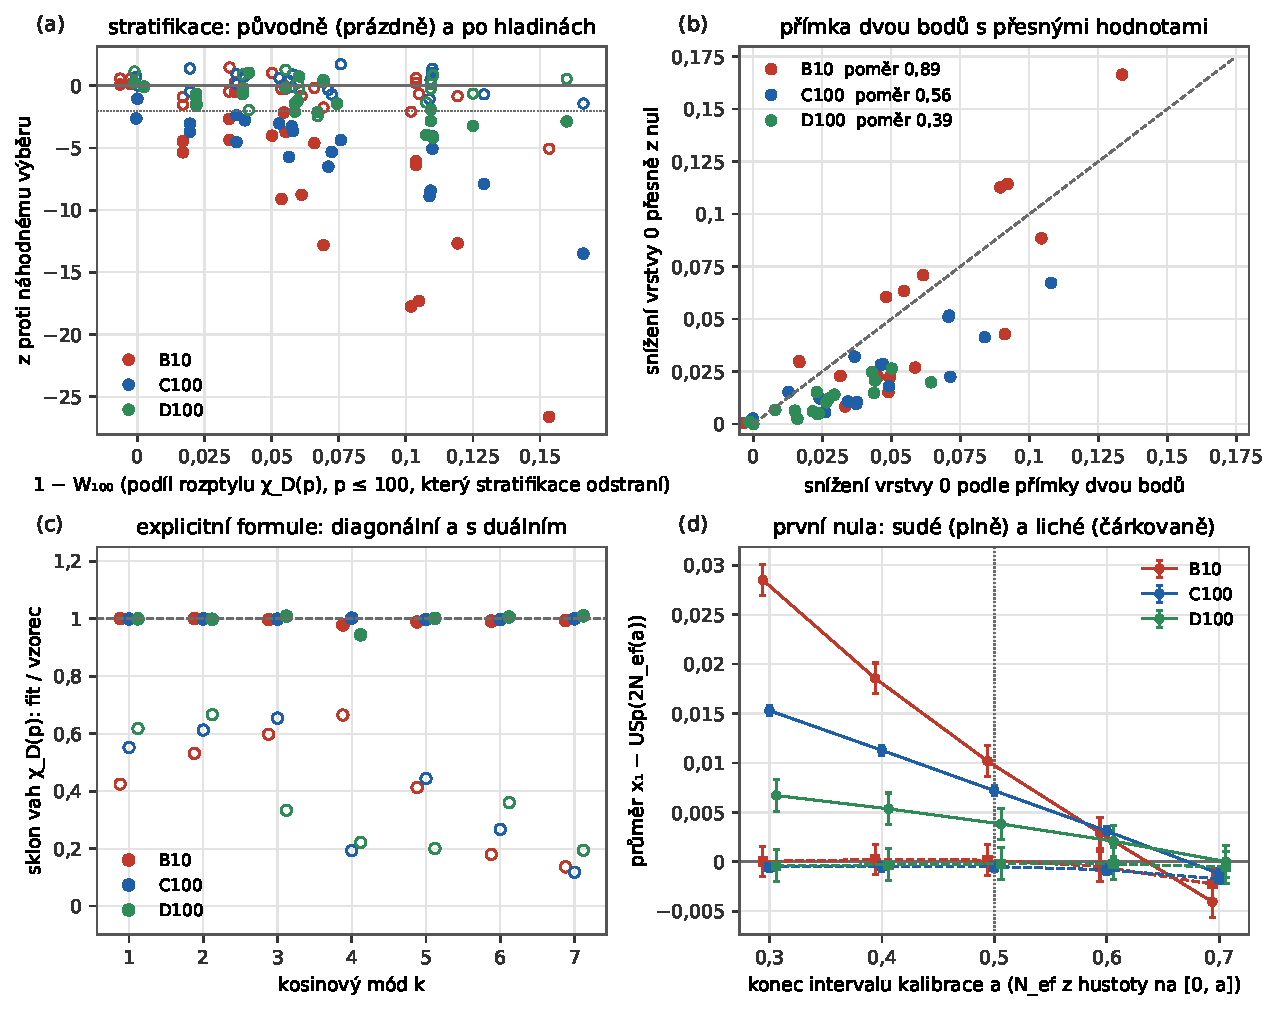
\includegraphics[width=0.95\textwidth,height=\textheight]{../../figures/09_recomputation_cz.pdf}
\caption{Obrázek 9. Přepočet po hladinách. (a) \(z\) 20 stratifikací
proti náhodným výběrům, původně (oddíl 4.4, prázdně) a po hladinách
(plně), proti podílu \(1 - W_{100}\) rozptylu \(\chi_D(p)\),
\(p \le 100\), který stratifikace odstraní. (b) Snížení vrstvy 0
stratifikacemi, přesně z nul, proti přímce dvěma body; čárkovaně
rovnost, v legendě střední poměr. (c) Sklon fitovaných vah \(\chi_D(p)\)
proti explicitní formuli po kosinových módech, jen diagonální členy
(prázdně) a s duálním členem domněnky poměrů (plně). (d) Průměr první
nuly minus USp\((2N_{\mathrm{ef}}(a))\) s \(N_{\mathrm{ef}}\) určeným
hustotou domněnky poměrů na \([0, a]\), sudé (plně) a liché (čárkovaně)
charaktery; tečkovaně \(a = \frac12\), kalibrace oddílu 4.5.}
\end{figure}

\hypertarget{zvux11btux161enuxed-u-d-1010-rodina-e100}{%
\subsection{\texorpdfstring{4.8 Zvětšení u \(|D| = 10^{10}\): rodina
E100}{4.8 Zvětšení u \textbar D\textbar{} = 10\^{}\{10\}: rodina E100}}\label{zvux11btux161enuxed-u-d-1010-rodina-e100}}

U největšího vodiče určoval chyby počet L-funkcí, ne počet nul: E10 jich
má 12 153. Rodina proto pokračuje bez překryvu až do
\(|D| = 10^{10} + 2\cdot10^5\): dalších 109 404 L-funkcí v 900 blocích
se 471 278 nulami, spočtených na druhém počítači touž revizí generátoru
(SHA-256 \texttt{e4a8325f…}, PARI/GP 2.17.2, krok hledání střední
rozestup / 8 jako u všech ostatních rodin) za 14 hodin na devíti
procesech; každý blok souhlasí se svým kontrolním součtem. Spolu s E10
tvoří rodinu E100 tohoto oddílu: všech 121 557 základních diskriminantů
s \(10^{10} < |D| < 10^{10} + 2\cdot10^5\) (60 772 sudých, 60 785
lichých), desetkrát víc než E10 při stejném \(l = 21{,}88\). Skripty
oddílů 4.1--4.7 proběhly na E100 beze změny (volba
\texttt{-\/-families\ E100}); dřívější oddíly a jejich čísla zůstávají,
jak jsou.

Rodina E10 a rodina E100 u \(|D| = 10^{10}\): \(\chi^2\) na koš 0,05
jednohladinové hustoty proti modelům (u domněnky poměrů vše / sudé /
liché), hustota v \([0, \frac12]\), průměr první nuly minus
USp\((2N_{\mathrm{ef}})\) (\(N_{\mathrm{ef}}\) na \([0, \frac12]\)) a
vzdálenost KS dělená kritickou hodnotou (5 \%).

{\small\begin{longtable}[]{@{}
  >{\raggedright\arraybackslash}p{(\columnwidth - 4\tabcolsep) * \real{0.3333}}
  >{\raggedright\arraybackslash}p{(\columnwidth - 4\tabcolsep) * \real{0.3333}}
  >{\raggedright\arraybackslash}p{(\columnwidth - 4\tabcolsep) * \real{0.3333}}@{}}
\toprule\noalign{}
\begin{minipage}[b]{\linewidth}\raggedright
\end{minipage} & \begin{minipage}[b]{\linewidth}\raggedright
E10
\end{minipage} & \begin{minipage}[b]{\linewidth}\raggedright
E100
\end{minipage} \\
\midrule\noalign{}
\endhead
\bottomrule\noalign{}
\endlastfoot
L-funkce (sudé / liché) & 12 153 (6 084 / 6 069) & 121 557 (60 772 / 60
785) \\ \addlinespace[2pt]
\(\chi^2\), domněnka poměrů & 0,661 / 0,813 / 0,835 & 0,759 / 0,785 /
0,821 \\ \addlinespace[2pt]
\(\chi^2\), bez \(A\) a \(\Delta\) & 2,57 & 16,48 \\ \addlinespace[2pt]
\(\chi^2\), USp\((2N)\), \(N = l/2\) & 3,42 & 24,44 \\ \addlinespace[2pt]
\(\chi^2\), USp & 7,81 & 66,75 \\ \addlinespace[2pt]
hustota v \([0, \frac12]\) (domněnka poměrů 0,5267, USp 0,4105) &
\(0{,}5273 \pm 0{,}0093\) & \(0{,}5291 \pm 0{,}0030\) \\ \addlinespace[2pt]
\(x_1 - {}\)USp\((2N_{\mathrm{ef}})\), sudé & \(+0{,}0013 \pm 0{,}0037\)
& \(+0{,}0016 \pm 0{,}0012\) \\ \addlinespace[2pt]
\(x_1 - {}\)USp\((2N_{\mathrm{ef}})\), liché &
\(-0{,}0017 \pm 0{,}0037\) & \(-0{,}0009 \pm 0{,}0012\) \\ \addlinespace[2pt]
KS / kritická hodnota, sudé / liché & 0,34 / 0,37 & 0,73 / 0,46 \\ \addlinespace[2pt]
\end{longtable}}

\textbf{Jednohladinová hustota.} I s desetinásobkem dat hustota sleduje
domněnku poměrů: \(\chi^2\) na koš 0,759, kdežto bez aritmetického
faktoru \(A\) a členu s \(\Delta\) je 16,5, proti USp\((2N)\) s
\(N = l/2\) 24,4 a proti limitě Katze a Sarnaka 66,7 (E10: 2,6, 3,4 a
7,8). Hustota v \([0, \frac12]\) je \(0{,}5291 \pm 0{,}0030\) proti
0,5267 podle domněnky poměrů a 0,4105 pro USp, 39 chyb nad limitou u
\(|D| = 10^{10}\). Jako souvislá rodina má E100 \(\chi^2\) pod 0,95, jak
dává čekat oddíl 4.3.

Souvislé úseky, stratifikace a explicitní formule podle vodiče, po
hladinách (oddíl 4.7): poměr jednoho úseku 6 074 po sobě jdoucích
diskriminantů přes všechny začátky k náhodným výběrům (přesně), snížení
stratifikací \(D \bmod 840\) se \(z\), počet z 19 modulů víc než 3 chyby
pod náhodnými výběry, přesné snížení vrstvy 0 stratifikacemi vůči přímce
dvou bodů, podíl přesného snížení jednoho úseku předpovězený jen z
charakterů (prvočíslo po prvočísle, s duálním členem) a sklon vah
\(\chi_D(p)\) s duálním členem (v závorce jen diagonální členy).

{\small\begin{longtable}[]{@{}
  >{\raggedright\arraybackslash}p{(\columnwidth - 14\tabcolsep) * \real{0.1250}}
  >{\raggedright\arraybackslash}p{(\columnwidth - 14\tabcolsep) * \real{0.1250}}
  >{\raggedright\arraybackslash}p{(\columnwidth - 14\tabcolsep) * \real{0.1250}}
  >{\raggedright\arraybackslash}p{(\columnwidth - 14\tabcolsep) * \real{0.1250}}
  >{\raggedright\arraybackslash}p{(\columnwidth - 14\tabcolsep) * \real{0.1250}}
  >{\raggedright\arraybackslash}p{(\columnwidth - 14\tabcolsep) * \real{0.1250}}
  >{\raggedright\arraybackslash}p{(\columnwidth - 14\tabcolsep) * \real{0.1250}}
  >{\raggedright\arraybackslash}p{(\columnwidth - 14\tabcolsep) * \real{0.1250}}@{}}
\toprule\noalign{}
\begin{minipage}[b]{\linewidth}\raggedright
rodina
\end{minipage} & \begin{minipage}[b]{\linewidth}\raggedright
\(l\)
\end{minipage} & \begin{minipage}[b]{\linewidth}\raggedright
úsek / náhodný
\end{minipage} & \begin{minipage}[b]{\linewidth}\raggedright
\(D \bmod 840\)
\end{minipage} & \begin{minipage}[b]{\linewidth}\raggedright
modulů pod \(-3\)
\end{minipage} & \begin{minipage}[b]{\linewidth}\raggedright
strata / přímka
\end{minipage} & \begin{minipage}[b]{\linewidth}\raggedright
z charakterů
\end{minipage} & \begin{minipage}[b]{\linewidth}\raggedright
sklon vah
\end{minipage} \\
\midrule\noalign{}
\endhead
\bottomrule\noalign{}
\endlastfoot
B10 & 9,62 & 0,204 & 17,2 \% (\(-26{,}6\)) & 15 & 0,89 & 89 \% & 0,995
(0,523) \\ \addlinespace[2pt]
C100 & 13,06 & 0,391 & 9,5 \% (\(-13{,}5\)) & 16 & 0,56 & 76 \% & 0,999
(0,578) \\ \addlinespace[2pt]
D100 & 17,28 & 0,606 & 1,6 \% (\(-2{,}9\)) & 3 & 0,39 & 65 \% & 0,999
(0,598) \\ \addlinespace[2pt]
E100 & 21,88 & 0,622 & 2,2 \% (\(-4{,}0\)) & 2 & 0,20 & 42 \% & 1,001
(0,608) \\ \addlinespace[2pt]
\end{longtable}}

\textbf{Souvislé úseky a zbytkové třídy.} Jeden úsek 6 074 po sobě
jdoucích diskriminantů si přes všech 115 484 začátků ponechá 0,622
výkonu nízkých módů náhodných výběrů (přesně, bez losování): jev
souvislých rodin trvá i u \(10^{10}\) a mezi \(10^8\) a \(10^{10}\)
skoro neslábne (0,606 → 0,622), přestože průměry \(\chi_D(p)\),
\(p \le 100\), si přes úsek ponechají jen 4,3 \% náhodného rozptylu
(\(W_{100}\)). Stratifikace se chovají jako v D100: \(D \bmod 840\)
sníží výkon o 2,2 \% (\(z = -4{,}0\)), dva z 19 modulů leží víc než 3
chyby pod; přímka dvou bodů neplatí (\(\chi^2 = 218\) pro 20) a přesné
snížení je 0,20 přímky, v řadě 0,89 / 0,56 / 0,39. Explicitní formule s
duálním členem popíše E100 jako ostatní rodiny (sklon
\(1{,}0007 \pm 0{,}0027\), \(\chi^2\) na koeficient 0,92; jen diagonální
členy 0,608), ale část snížení jednoho úseku, kterou dají charaktery
prvočíslo po prvočísle, s vodičem klesá, 89 / 76 / 65 / 42 \%; zbytek,
který předpověď prvočíslo po prvočísle neobsahuje (součiny
\(\chi_D(p)\chi_D(q)\), oddíl 4.6), s \(l\) roste.

\textbf{První nula.} Liché charaktery souhlasí s
USp\((2N_{\mathrm{ef}})\) i při třikrát menší chybě
(\(-0{,}0009 \pm 0{,}0012\), KS 0,46 kritické hodnoty). U sudých
charakterů je posun průměru (\(N_{\mathrm{ef}}\) na \([0, \frac12]\),
oddíl 4.5) \(+0{,}0016 \pm 0{,}0012\), 2,3 chyby pod hodnotou 0,0043
zákona \(0{,}094/l\), který oddíl 4.5 fitoval na B10, C100, R10, D100 a
E10 (E10 měla chybu 0,0037). S E100 místo E10 je \(c/l\) stále
přijatelné (\(p = 0{,}17\)), ale volná mocnina \(c\,l^{-a}\) dá
\(a = 1{,}60\) (1,27--1,95) místo 1,33 (0,91--1,74) a data mezi \(1/l\)
a \(1/l^2\) nerozhodnou. Odchylka tvaru je zřetelnější. U \(x_1 = 1\) je
rozdíl \(F(1) - \mathrm{USp}(2N_{\mathrm{ef}})\) sudých charakterů v
E100 \(-0{,}0029 \pm 0{,}0015\) proti \(-0{,}0069\) z mocninného zákona
fitovaného na B10, C100, R10 a D100 (\(a = 1{,}34\); 2,7 chyby) a jedna
mocnina už všech pět rodin nepopíše (\(p = 0{,}09\); \(1/l\):
\(p = 0{,}003\), \(1/l^2\): \(p = 0{,}04\)). Při kalibraci
\(N_{\mathrm{ef}}\) na \([0, a]\) zůstává vzdálenost KS sudých
charakterů pod kritickou hodnotou při každé kalibraci (0,56--0,89 z ní)
a posun průměru jde od \(+0{,}0026\) (\(a = 0{,}3\)) k \(+0{,}0000\)
(\(a = 0{,}7\)) (obrázek 10 vpravo dole). U \(10^{10}\) je člen sudých
charakterů na mezi rozlišení 60 000 L-funkcí (1,3 a 1,9 chyby) a podle
vodiče klesá mezi \(l = 17\) a \(22\) rychleji než \(1/l\). Zda jde o
jev konečné velikosti při srovnání s jediným USp\((2N_{\mathrm{ef}})\),
nebo o vlastnost rodiny, vyžaduje první nulu z domněnky poměrů
(otevřené).

Zvětšení potvrzuje oddíly 4.1--4.7 u \(10^{10}\) s asi třikrát menšími
chybami a mění jedno tvrzení: zákon \(0{,}094/l\) posunu sudých
charakterů (oddíl 4.5) už není preferovaný a odchylka tvaru klesá
rychleji než \(1/l\).

\begin{figure}
\centering
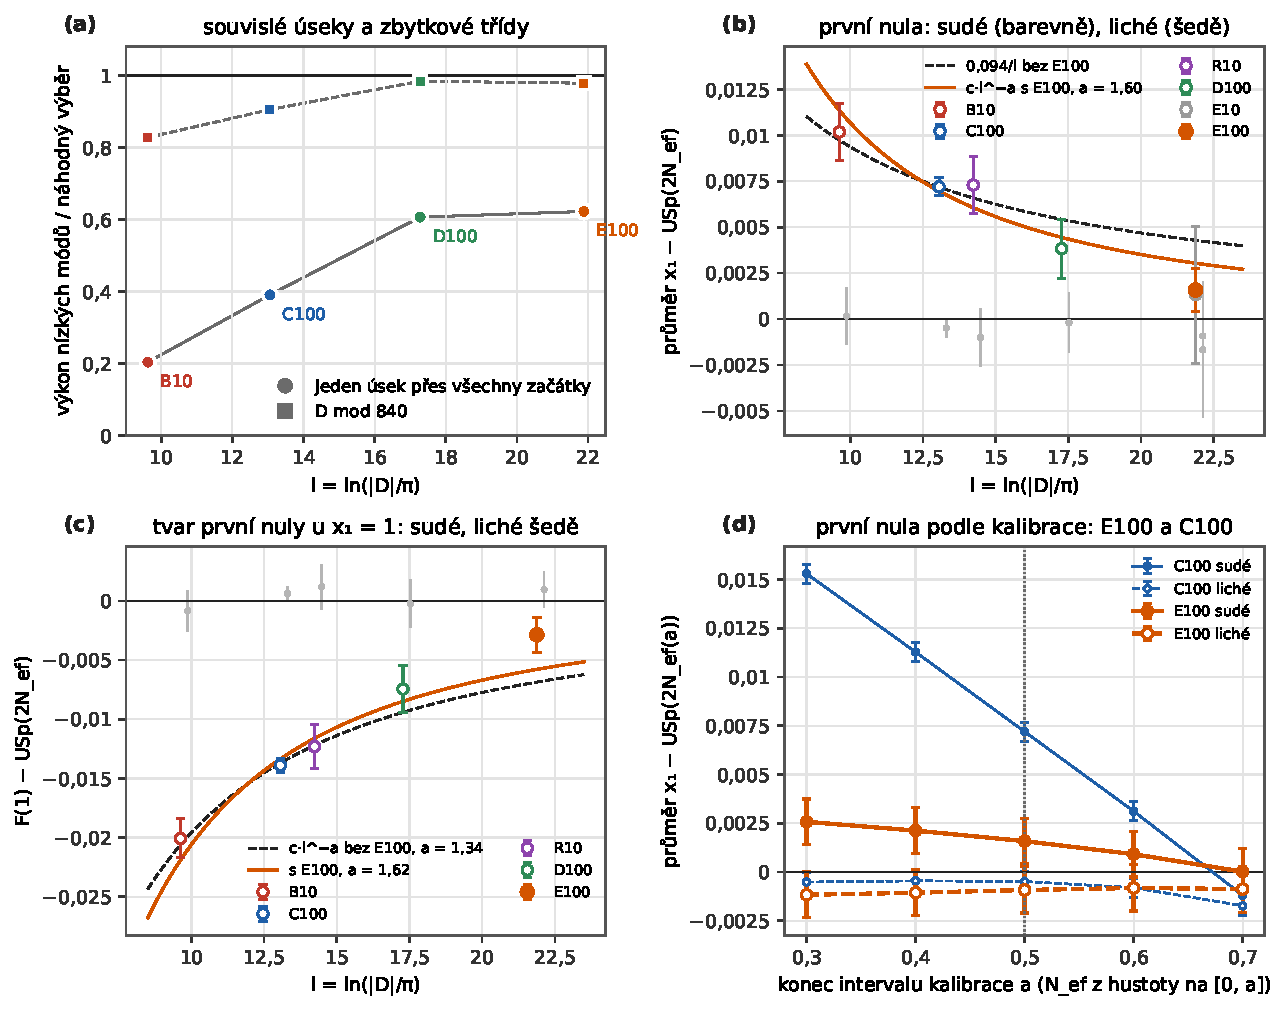
\includegraphics[width=0.95\textwidth,height=\textheight]{../../figures/10_e100_cz.pdf}
\caption{Obrázek 10. Zvětšení u \(|D| = 10^{10}\) (rodina E100, 121 557
L-funkcí). (a) Výkon nízkých módů jednoho souvislého úseku přes všechny
začátky (kroužky) a výběrů stratifikovaných podle \(D \bmod 840\)
(čtverce) vůči náhodným výběrům, po hladinách. (b) Posun průměru první
nuly sudých charakterů proti USp\((2N_{\mathrm{ef}})\)
(\(N_{\mathrm{ef}}\) na \([0, \frac12]\)) podle \(l = \ln(|D|/\pi)\);
prázdně rodiny oddílu 4.5, plně E100; čárkovaně zákon \(0{,}094/l\) bez
E100, plně \(c\,l^{-a}\) s E100; liché charaktery šedě. (c) Odchylka
tvaru, \(F(1) - \mathrm{USp}(2N_{\mathrm{ef}})\) u \(x_1 = 1\), pro sudé
charaktery s \(c\,l^{-a}\) fitovaným bez E100 (čárkovaně) a s E100
(plně); liché šedě. (d) Průměr první nuly minus
USp\((2N_{\mathrm{ef}}(a))\) při kalibraci \(N_{\mathrm{ef}}\) na
\([0, a]\), E100 (silně) a C100 (slabě), sudé (plně) a liché (prázdně).}
\end{figure}

\hypertarget{tvrzenuxed-a-jejich-stav}{%
\section{5. Tvrzení a jejich stav}\label{tvrzenuxed-a-jejich-stav}}

{\small\begin{longtable}[]{@{}
  >{\raggedright\arraybackslash}p{(\columnwidth - 2\tabcolsep) * \real{0.5435}}
  >{\raggedright\arraybackslash}p{(\columnwidth - 2\tabcolsep) * \real{0.4565}}@{}}
\toprule\noalign{}
\begin{minipage}[b]{\linewidth}\raggedright
tvrzení
\end{minipage} & \begin{minipage}[b]{\linewidth}\raggedright
stav
\end{minipage} \\
\midrule\noalign{}
\endhead
\bottomrule\noalign{}
\endlastfoot
Jednohladinovou hustotu nízko položených nul kvadratických
Dirichletových L-funkcí při konečném vodiči dává domněnka poměrů (tvar
Conreyho a Snaithové, přizpůsobený všem základním diskriminantům). &
Známá teorie {[}8, 9{]}, domněnková; zde v souladu s 795 381 L-funkcemi
v jedenácti rodinách do \(|D| = 10^{10}\), \(\chi^2\) na koš 0,54--1,19,
hustota u středového bodu do 1,2 chyby ve 33 kombinacích; u
\(|D| = 10^{10}\) i se 121 557 L-funkcemi rodiny E100 (\(\chi^2\) 0,759,
oddíl 4.8). \\ \addlinespace[2pt]
Limity Katze a Sarnaka USp se při těchto vodičích nedosáhne. & Známé
{[}7, 9{]}; zde změřeno: při \(|D| = 10^{10}\) je hustota v
\([0; \frac12]\) o 12,6 chyby nad USp a sleduje domněnku poměrů pro
jeden diskriminant; v E100 39 chyb (oddíl 4.8). \\ \addlinespace[2pt]
Rodiny po sobě jdoucích diskriminantů mají menší kolísání hustoty na
nízkých frekvencích \(u < \ln\Delta/\ln(|D|/\pi)\) než náhodné výběry,
protože průměry \(\chi_D(p)\) pro \(p\) pod délkou úseku \(\Delta\)
procházejí téměř úplné periody. & Zde změřeno (0,23 / 0,36 / 0,48 výkonu
na nízkých frekvencích při \(|D| \approx 5\cdot10^4\) /
\(1{,}5\cdot10^6\) / \(10^8\); 5,9 / 10,2 / 4,3 chyby); mechanismus je
periodicita používaná ve větách o středních hodnotách {[}14, 15{]} a
\(u_c\) je obdobou přechodu při nosiči 1 pro krátkou rodinu {[}7, 16,
17{]}; testováno podmnožinami z \(m\) kusů. Pokud jsme mohli zjistit,
velikost jevu pro souvislé podrodiny dosud nebyla kvantifikována. \\ \addlinespace[2pt]
Nízké \(\chi^2\) rodiny \(10^4 < |D| \le 2\cdot10^4\) je výjimečné. &
Zde zamítnuto: je to nejnižší z devíti souvislých pásem, 1,5 směrodatné
odchylky pod jejich průměrem. \\ \addlinespace[2pt]
Nízké \(\chi^2\) způsobuje vyrovnání zbytkových tříd \(D\) modulo
nejmenší prvočísla. & Zde zamítnuto pro 19 modulů (3 \ldots{} 840 a 131)
a znaménko, s nezávislým opakováním: v C100 a D100 žádná stratifikace
nad náhodu, v B10 jen \(D \bmod 840\) (\(z = -5{,}1\)); vyrovnání
\(D \bmod 8\) (\(\chi_D(2)\)) ani znaménka nerozhoduje. Oddíl 4.7, po
hladinách: každý modul přesnou vrstvu 0 mírně sníží, o víc než 3 chyby u
15 / 16 / 3 z 19 modulů v B10 / C100 / D100; \(D \bmod 840\) odebere 17
/ 9,5 / 1,6 \% náhodné hodnoty proti 79 / 64 / 50 \% u pásem, takže
zamítnutí platí. \\ \addlinespace[2pt]
Stratifikace podle \(D \bmod M\) ustálí průměry \(\chi_D(p)\) jen pro
prvočísla dělící \(M\) (pro \(p = 2\) jen při \(8 \mid M\)). & Zde v
souladu (elementární periodicita): přesný rozptyl stratifikovaného
výběru je pro \(p \mid M\) nejvýš 0,07 náhodného rozptylu a pro ostatní
prvočísla 1,000--1,014; náhodné výběry souhlasí s výběrem z konečného
souboru do 0,4 \%. \\ \addlinespace[2pt]
Výkon nul podmnožiny na nízkých frekvencích sleduje zbylý rozptyl \(W\)
součtů \(\chi_D(p)\) přes malá prvočísla. & Zde změřeno: ve směru pro
všech 60 stratifikovaných podmnožin; ve velikosti jen na hraně ---
\(\chi^2 = 82{,}05\) pro 60 se společnými chybami (\(p = 0{,}03\)), 42 z
60 odchylek kladných. Pokud jsme mohli zjistit, dosud nepopsáno. Oddíl
4.7: s hodnotami po hladinách ve velikosti zamítnuto
(\(\chi^2 = 841{,}8\) pro 60, \(p < 10^{-130}\)); přesně dávají
stratifikace 0,89 / 0,56 / 0,39 snížení přímky. \\ \addlinespace[2pt]
Stejné váhy \((\ln p)^2/p\) pro všechna prvočísla nízkých módů předpoví
velikost. & Zde zamítnuto: posun odchylek zmizí, ale \(\chi^2 = 91{,}0\)
pro 60 (\(p = 0{,}006\)) a B10 mod 840 leží 4,1 chyby pod předpovědí. \\ \addlinespace[2pt]
Podíl \(W_k\) profilu pásem vážený \(k\) předpoví velikost závislosti
souvislých pásem na vodiči. & Zde zamítnuto: pořadí souhlasí (\(W_k\)
0,22 → 0,61 → 0,70, naměřený poměr 0,22 → 0,38 → 0,49), velikost pro
C100 se liší o 7 chyb; otevřené. Oddíl 4.7: přesný poměr 0,204 / 0,391 /
0,606. \\ \addlinespace[2pt]
USp\((2N)\) s \(N = \frac12\ln(|D|/\pi)\) popíše první nulu. & Zde
zamítnuto (KS 1,6× až 53× kritické hodnoty). \\ \addlinespace[2pt]
USp\((2N_{\mathrm{ef}})\) s \(N_{\mathrm{ef}}\) z domněnky poměrů dává
první nulu lichých charakterů. & Zde v souladu při všech vodičích od
\(10^3\) do \(10^{10}\), KS všude pod kritickou hodnotou. \\ \addlinespace[2pt]
Totéž platí pro sudé charaktery. & Zde zamítnuto: 14,8 chyby v C100;
odchylka klesá zhruba jako \(0{,}094/\ln(|D|/\pi)\). Oddíl 4.7: posun
průměru závisí na intervalu kalibrace \(N_{\mathrm{ef}}\) (pro
\([0; 0{,}7]\) nejvýš 0,0041); odchylka tvaru (KS) zůstává v B10 a C100
při každé kalibraci. Oddíl 4.8: v E100 (121 557 L) je posun
\(+0{,}0016 \pm 0{,}0012\), 2,3 chyby pod \(0{,}094/l\); s E100 dá volná
mocnina \(l^{-a}\) \(a = 1{,}60\) (1,27--1,95) a odchylka tvaru u
\(x_1 = 1\) klesá rychleji než \(1/l\) (\(p = 0{,}003\)). \\ \addlinespace[2pt]
Očekávaný výkon nízkých frekvencí podmnožiny se dá spočítat bez losování
(chyba z očekávaného počtu) a statistika testu se od něj liší jen malým
rozdílem, který stačí losovat. & Odvozeno a změřeno zde: losovaná
Pearsonova statistika = vrstva 0 do \(10^{-6}\), chyba bodu 3,6 / 3,8 /
4,1× menší. \\ \addlinespace[2pt]
Posun kolem 5 \% mezi statistikou testu a očekávanou hodnotou je náhodný
šum. & Zamítnuto zde: kladný u všech 30 návrhů (6,2 / 8,7 / 3,8 chyb);
je to zkreslení chyby z pozorovaného počtu ve dvou nejnižších koších (84
\% v B10). \\ \addlinespace[2pt]
Trojice po sobě jdoucích diskriminantů mají menší výkon nízkých
frekvencí než náhodný výběr. & Změřeno zde v B10 a C100 (0,972 / 0,975,
4,7 / 4,3 chyby), jak předpoví vrstva 0; v D100 pod rozlišením. \\ \addlinespace[2pt]
Módy \(k\) a \(8 - k\) příspěvku jedné L-funkce jsou spřažené a vazba je
druhého řádu v charakterech (součiny \(\chi_D(p)\chi_D(q)\) nesou módy
6--7). & Změřeno zde: korelace 0,35--0,58 (Poisson 0), poměr módů 6--7 k
1--4 13,8 / 14,6 / 19,0, nulový model nejvýš 0,0003. Pokud víme, dosud
nepopsáno. \\ \addlinespace[2pt]
Rozdíl první nuly sudých charakterů a USp\((2N_{\mathrm{ef}})\) mění
znaménko v \(x_1 = \frac12\). & Jako vlastnost nul zamítnuto: naměřeno
\(0{,}508 \pm 0{,}021\) (C100) a \(0{,}488 \pm 0{,}038\) (B10), průsečík
ale sleduje konec \(a\) intervalu, na kterém se určuje
\(N_{\mathrm{ef}}\) (sklon 1,13 a 1,15 pro \(a = 0{,}3\)--\(0{,}7\),
nejvýš 0,071 od \(a\)). \\ \addlinespace[2pt]
Souvislý úsek šířky \(\Delta\) je dolní propust ve frekvenci prvočísel
do \(u_c = \ln\Delta/l\) (obdoba nosiče \(|u| < 1\) testovacích funkcí
celé rodiny); stratifikace podle \(D \bmod 840\) je hřebenový filtr na
prvočíslech 2, 3, 5, 7 a jejich součinech. & V souladu zde (heuristika s
nerovností Pólyi--Vinogradova, ne věta): poměr úseku a náhodného výběru
pod / nad \(k_c\) v C100 0,20--0,43 / 0,44--0,54; rozklad mod 840 bez
losování, součiny 33 / 24 / 17 \% snížení. \\ \addlinespace[2pt]
Každé číslo oddílů 4.3--4.5 z náhodných podmnožin se dá přepočítat se
stejnými návrhy, s přesnou vrstvou 0 a losováním jen rozdílu (oddíl
4.7). & Odvozeno a změřeno zde: 84 návrhů, kontrola vrstvy 0 se středním
\(z^2\) 1,13 a \(|z| \le 3{,}0\); chyba výkonu nízkých frekvencí
1,6--4,6× menší (medián 3,7); původní hodnoty souhlasí v rámci
společných chyb (63 hodnot, nejvíc 2,3 chyby). \\ \addlinespace[2pt]
V C100 a D100 žádná stratifikace nemění výkon nízkých frekvencí nad
náhodu; v B10 jen \(D \bmod 840\) (oddíl 4.4). & Po hladinách zde
zamítnuto (oddíl 4.7): o víc než 3 chyby u 15 / 16 / 3 z 19 modulů;
účinek je malý (17 / 9,5 / 1,6 \% u \(D \bmod 840\)). \\ \addlinespace[2pt]
Diagonální členy \(n = p^k\) explicitní formule dávají závislost
příspěvku jedné L-funkce na \(\chi_D(p)\). & Zde zamítnuto: sklon
fitovaných proti předpovězeným vahám 0,52 / 0,58 / 0,60; \(\chi^2\) 6
469 / 33 797 / 1 746 pro 30 koeficientů v oknech \(x\). \\ \addlinespace[2pt]
S duálním členem domněnky poměrů pro podrodinu \(\chi_D(p) = e\) jsou
váhy jednotlivých prvočísel úplné. & Odvozeno z domněnky poměrů {[}8,
9{]} a zde v souladu: sklon 0,995 / 0,999 / 0,999, \(\chi^2\) na
koeficient 0,45 / 0,31 / 0,78. \\ \addlinespace[2pt]
Snížení stratifikacemi a úseky plyne ze samotných charakterů, po
prvočíslech. & Částečně: \(D \bmod 8\) s přesností 3 \%, \(D \bmod 840\)
54--104 \%, jeden úsek 65--89 \% přesného snížení; součiny
\(\chi_D(p)\chi_D(q)\) nejsou zahrnuty; otevřené. \\ \addlinespace[2pt]
Posun průměru první nuly sudých charakterů je vlastnost nul. & Zde
zamítnuto: závisí na intervalu \([0, a]\), na kterém se
\(N_{\mathrm{ef}}\) určuje, a mění znaménko mezi \(a = 0{,}6\) a 0,7 v
B10, C100 a E10. \\ \addlinespace[2pt]
Dvouhladinová část \(P(x_1 \le a)\) je do \(a = \frac12\) zanedbatelná.
& Změřeno zde: nejvýš 0,0002 v USp\((2N_{\mathrm{ef}})\) a 0,00007 v
datech, takže \(F(\frac12)\) určuje jednohladinová hustota. \\ \addlinespace[2pt]
Hledání v datech najde každou nulu do \(x = 4{,}3\). & Zde zamítnuto, v
malé míře: z 3 000 L-funkcí na rodinu chybí jedné v B10 dvojice blízkých
nul (\(x\) = 3,31 a 3,33), v C100 žádné; relativní úbytek řádu
\(10^{-4}\). \\ \addlinespace[2pt]
Jev souvislých rodin s vodičem slábne. & Zde změřeno (oddíl 4.8): jeden
úsek si ponechá 0,204 / 0,391 / 0,606 / 0,622 výkonu nízkých módů
náhodných výběrů při \(l\) = 9,6 / 13,1 / 17,3 / 21,9; mezi \(10^8\) a
\(10^{10}\) se skoro nemění, kdežto podíl jeho snížení, který dají
jednotlivá prvočísla, klesá z 89 na 42 \%. \\ \addlinespace[2pt]
Odchylka tvaru první nuly sudých charakterů klesá jako
\(1/\ln(|D|/\pi)\). & Zde zamítnuto (oddíl 4.8):
\(F(1) - \mathrm{USp}(2N_{\mathrm{ef}}) = -0{,}0029 \pm 0{,}0015\) v
E100 proti \(-0{,}0069\) z B10--D100 (2,7 chyby); pro \(1/l\)
\(p = 0{,}003\); v E100 je vzdálenost KS pod kritickou hodnotou při
každé kalibraci. \\ \addlinespace[2pt]
\end{longtable}}

\hypertarget{co-je-novuxe9-a-co-je-potvrzenuxe9}{%
\section{6. Co je nové a co je
potvrzené}\label{co-je-novuxe9-a-co-je-potvrzenuxe9}}

\textbf{Potvrzené: známá teorie, zde změřená ve větším rozsahu.} (i)
Jednohladinová hustota při konečném vodiči sleduje domněnku poměrů {[}8,
9{]}; dřívější numerické testy této rodiny provedli Rubinstein {[}7{]},
Miller {[}10{]} a Stopple {[}18{]} (jeden úsek asi \(10^6\)
diskriminantů u \(10^{12}\)), zde na 795 381 L-funkcích v jedenácti
rodinách s nulovými modely, bootstrapem a nezávislou kontrolou. (ii)
Limity Katze a Sarnaka se při těchto vodičích nedosáhne {[}7, 9{]}.
(iii) Efektivní velikost matice zlepší popis první nuly, jako u
\(\zeta\) {[}11{]} a u eliptických křivek {[}12{]}. (iv) \(\chi_D(p)\)
je v \(D\) periodické, což je základ vět o středních hodnotách přes
diskriminanty {[}14, 15{]}; průměry \(\chi_D(p)\) přes rozmezí \(D\)
jsou předmětem literatury o murmuracích {[}15, 16, 19{]}.

\textbf{Nové, pokud jsme mohli zjistit.} Hledali jsme na arXivu a v
časopisech (3. listopadu 2026) numerické testy kvadratických rodin,
murmurace a jejich vztah k domněnkám poměrů {[}15, 16, 19{]}, členy
nižšího řádu {[}10, 17{]} a rozptyl statistik rodiny přes podrodiny.
Stopple {[}18{]} používá jedno souvislé rozmezí a podmnožiny nesrovnává;
Cowan {[}19{]} spojuje murmurace s domněnkami poměrů přes průměry, ne
přes rozptyl podmnožin. Nenašli jsme: (a) že souvislé podrodiny mají
měřitelně menší kolísání jednohladinové hustoty na nízkých frekvencích
než náhodné výběry (0,23 / 0,36 / 0,48 výkonu), potlačené pod
\(u_c = \ln\Delta/\ln(|D|/\pi)\) a postupně ztracené podmnožinami z
\(m\) kusů (oddíl 4.3); (b) že vyrovnání zbytkových tříd podle
kteréhokoli z 19 modulů ho nevytvoří (oddíl 4.4); (c) že zbylý rozptyl
součtů charakterů, spočtený bez nul, seřadí výkon nul na nízkých
frekvencích všech 60 stratifikovaných podmnožin a souvislých pásem podél
jedné přímky, ve směru a ve velikosti na hraně (oddíl 4.4); (d) že
profil \(r_p\) souvislých pásem je táž funkce \(p\) ve třech rodinách od
\(|D| = 10^4\) do \(10^8\) (oddíl 4.4); (e) že pro sudé charaktery leží
první nula nad USp\((2N_{\mathrm{ef}})\) asi o \(0{,}094/\ln(|D|/\pi)\),
pro liché ne (oddíl 4.5); (f) že očekávaný výkon podmnožin jde spočítat
bez losování a že posun testu o několik procent je zkreslení dvou
nejnižších košů, ne šum a (g) že vazbu módů \(k \leftrightarrow 8 - k\)
nesou součiny charakterů malých prvočísel (intermodulace) (oddíl 4.6); a
(h) test domněnky poměrů na úrovni jednotlivých prvočísel: závislost nul
jedné L-funkce na \(\chi_D(p)\) sleduje diagonální členy explicitní
formule jen spolu s duálním členem (sklon 0,995--0,999 místo 0,52--0,60;
oddíl 4.7); a (i) u \(|D| = 10^{10}\) se 121 557 L-funkcemi, že jev
souvislých rodin trvá (0,62 výkonu náhodných výběrů), kdežto část nesená
jednotlivými prvočísly se zmenšuje, a že člen sudých charakterů u první
nuly klesá rychleji než \(1/\ln(|D|/\pi)\) (oddíl 4.8).

\textbf{Otevřené.} Velikost závislosti na vodiči v (a) a účinku
stratifikací v (c) (oddíl 4.4) a odvození členu sudých charakterů v (e)
z domněnky poměrů pro první nulu. Odvození vazby módů z explicitního
vzorce pro jednu L-funkci je otevřené. Oddíl 4.7 přidává tu část snížení
stratifikacemi a úseky, kterou charaktery po prvočíslech nedají (součiny
\(\chi_D(p)\chi_D(q)\)), a tvar první nuly sudých charakterů, který se
odchyluje při každé kalibraci, kdežto posun jejího průměru ne. Oddíl 4.8
přidává, proč člen sudých charakterů klesá rychleji než \(1/l\) a proč
podíl jednotlivých prvočísel na snížení úseků s vodičem klesá.

\hypertarget{diskuse}{%
\section{7. Diskuse}\label{diskuse}}

Kvadratická rodina se chová tak, jak říká domněnka poměrů, při každém
vodiči a na každém testovaném měřítku: v koších 0,025, 0,05 a 0,1, bez
košů, pro každé znaménko, u středového bodu i do čtyř středních
rozestupů. Její členy nižšího řádu nejsou při těchto vodičích malé
opravy; hustota u středového bodu je i při \(|D| = 10^{10}\) o čtvrtinu
nad hodnotou Katze a Sarnaka a model s konečnou maticí naivní velikosti
mine první nulu až o 15 \%.

Nízké \(\chi^2\) některých rodin, které vypadalo jako vlastnost nul, je
vlastnost výběru rodiny. Po sobě jdoucí diskriminanty jsou aritmeticky
pravidelný vzorek: pro každé prvočíslo pod délkou úseku nabývají
charaktery jednotlivých hodnot v téměř přesných poměrech a explicitní
vzorec tím vyhladí hustotu rodiny na odpovídajících nízkých frekvencích.
Pro numerickou práci s rodinami to má význam: \(\chi^2\) test souvislé
rodiny proti přesnému modelu má referenční hodnotu pod hodnotou pro
nezávislé L-funkce, o kolik, záleží na délce úseku a na vodiči; náhodné
výběry se tomu vyhnou. Těch 19 modulů to zostří: žádné uspořádání
zbytkových tříd nevytvoří to, co souvislost, protože modul ustálí jen
několik prvočísel, která ho dělí, kdežto nízké frekvence nesou všechna
prvočísla až do tisíců. Prakticky to znamená, že součty charakterů,
které nuly nepotřebují, už ukážou, které podrodiny budou kolísat méně a
zhruba o kolik; přesnou velikost dají až nuly.

První nula znaménka rozliší. Pro liché charaktery dává jediná efektivní
velikost matice, určená hustotou domněnky poměrů u středového bodu, celé
rozdělení první nuly v mezích chyb 300 000 L-funkcí; pro sudé mine o
člen relativní velikosti asi 1 \% při \(|D| \approx 10^6\), klesající
zhruba jako \(1/\ln|D|\). Znaménko vstupuje do explicitního vzorce gama
faktorem \(\Gamma((s + \kappa)/2)\) {[}10, 17{]}; velikost členu pro
první nulu jsme v literatuře nenašli. Eliptické křivky potřebovaly jiné
zpřesnění, vyříznutý soubor {[}12{]}. Bod, v němž sudá křivka protne
USp\((2N_{\mathrm{ef}})\), určuje kalibrace \(N_{\mathrm{ef}}\), ne nuly
(oddíl 4.5). Zda lze člen sudých charakterů odvodit z domněnky poměrů
pro první nulu (k tomu nestačí jednohladinová hustota), je otevřené.

Přepočet po hladinách (oddíl 4.7) zachovává hlavní závěr oddílů 4.3--4.5
--- nízké \(\chi^2\) souvislých rodin pochází ze samotného úseku,
zbytkové třídy vysvětlí jen malou část --- a upřesňuje velikosti.
Losovaná čísla souhlasí s přesnými v rámci svých chyb; mezí byly chyby.
Menší chyba změnila dvě tvrzení s omezeným rozlišením --- žádná
stratifikace nad náhodu v C100 a D100, přímka dvěma body na hraně --- v
naměřený malý účinek a zamítnutý zákon. Váhy explicitní formule ukazují,
kde zbylá struktura sedí: v duálním členu domněnky poměrů, který v
nízkých módech vyruší zhruba polovinu diagonální váhy, a v součinech
charakterů. U první nuly je rozdíl sudých a lichých v průměru věcí
kalibrace \(N_{\mathrm{ef}}\), rozdíl tvaru ne.

Zvětšení u \(|D| = 10^{10}\) (oddíl 4.8) ukazuje týž obraz u největšího
vodiče s asi třikrát menšími chybami. Nové jsou dva trendy. Jev
souvislých rodin mezi \(10^8\) a \(10^{10}\) neslábne (0,61 → 0,62
výkonu náhodných výběrů), kdežto část, kterou nesou jednotlivá malá
prvočísla, se zmenšuje (89 → 42 \% snížení jednoho úseku), takže u
velkých vodičů sedí jev stále víc v tom, co předpověď prvočíslo po
prvočísle vynechá. A člen sudých charakterů u první nuly klesá rychleji
než \(1/l\); u \(10^{10}\) je na mezi rozlišení, takže rozdíl tvaru
nalezený u menších vodičů ještě není tvrzením o limitě.

Nic z toho se netýká zobecněné Riemannovy hypotézy: nuly byly spočteny
na kritické přímce a testuje se jejich statistika.

\hypertarget{reprodukovatelnost}{%
\section{8. Reprodukovatelnost}\label{reprodukovatelnost}}

Skript \texttt{compute\_families.py} přepočítá každé číslo oddílů
4.1--4.3 a 4.5 z nul asi za pět minut a zapíše
\texttt{reference\_families.json}, \texttt{reference\_subsets.json} a
\texttt{reference\_pieces.json}; \texttt{figures.py} z nich nakreslí
všechny obrázky a \texttt{export\_csv.py} zapíše datové soubory;
\texttt{pieces\_repeat.py} (asi 4 minuty) zopakuje test kusy s 400
podmnožinami na bod a chybou každého bodu a zapíše
\texttt{reference\_pieces\_repeat.json} (obrázek 5 vpravo). Nuly vyrábí
\texttt{ks\_nuly.py} (PARI/GP; rodiny A, B, B10, C10, D10, E, R asi za
dvě hodiny na dvou jádrech, sadu C100, D100, E10, R10 asi za čtyři
hodiny na devíti jádrech) a lze je ověřit podle
\texttt{block\_content\_sha256.csv}; \texttt{ks\_kontrola.py}
zkontroluje úplnost rodiny bez PARI a \texttt{read\_zeros.py} čte bloky.
Skripty \texttt{compute\_moduli.py} (asi 8 minut) a
\texttt{character\_sums.py} (asi 20 minut; přesné rozptyly všech 20
stratifikací a profil pásem) spočtou oddíl 4.4 a zapíší
\texttt{reference\_moduli.json} a \texttt{reference\_characters.json};
\texttt{figures\_moduli.py} nakreslí obrázek 6 a \texttt{export\_csv.py}
zapíše také \texttt{moduli.csv}, \texttt{character\_sums.csv} a
\texttt{band\_profile.csv}. Skript \texttt{exact\_layers.py} (asi 40
minut) spočítá oddíl 4.6 (vrstvy, kusy, posun, vyvážené výběry, regrese,
vazbu módů) a zapíše \texttt{reference\_layers.json},
\texttt{intermodulation.py} (asi 2 minuty) intermodulaci a
\texttt{reference\_intermodulation.json},
\texttt{first\_zero\_crossing.py} (asi 20 sekund) průsečík první nuly s
testem kalibrace a \texttt{reference\_first\_zero\_crossing.json};
\texttt{figures\_layers.py} kreslí obrázek 8 a \texttt{export\_csv.py}
píše také \texttt{layers.csv}, \texttt{intermodulation.csv} a
\texttt{first\_zero\_crossing.csv}. Oddíl 4.7 počítají
\texttt{layered\_recomputation.py} (asi 25 minut na dvou jádrech; oddíly
4.3 a 4.4 po hladinách, \texttt{reference\_recomputation.json}),
\texttt{explicit\_weights.py} (asi 20 minut; váhy explicitní formule s
duálním členem, \texttt{reference\_explicit\_weights.json}),
\texttt{two\_level\_first\_zero.py} (asi minuta; dvouhladinová část a
kalibrace první nuly, \texttt{reference\_two\_level.json}) a
\texttt{missing\_zeros.py} (PARI/GP; asi 3 a 12 minut pro 3 000 L-funkcí
z B10 a C100, \texttt{reference\_missing\_zeros\_B10.json} a
\texttt{\_C100.json}); \texttt{figures\_recomputation.py} kreslí obrázek
9 a \texttt{export\_csv.py} píše také \texttt{recomputation.csv},
\texttt{recomputation\_line.csv}, \texttt{explicit\_weights.csv},
\texttt{two\_level.csv} a \texttt{missing\_zeros.csv}. Oddíl 4.8: tytéž
skripty s volbou \texttt{-\/-families\ E100}
(\texttt{compute\_families.py} 1. fáze,
\texttt{layered\_recomputation.py}, \texttt{two\_level\_first\_zero.py}
a \texttt{explicit\_weights.py}; dohromady asi 15 minut) zapíšou soubory
\texttt{…\_E100.json}; \texttt{e100\_trends.py} (sekundy) fituje trendy
podle vodiče (\texttt{reference\_e100\_trends.json}) a
\texttt{figures\_e100.py} nakreslí obrázek 10; nuly E100 znovu vytvoří
\texttt{ks\_nuly.py\ -\/-rodiny\ E100\ -\/-divz\ 8} (asi 128 hodin CPU).
Skript \texttt{independent\_check.py} nesdílí s ostatními žádný kód
(vlastní čtení, rozvinutí, předpověď jinou cestou, kosinová matice,
Fredholmova kvadratura a náhodné výběry, Hardyho funkce pro úplnost nul
a pro oddíl 4.4 vlastní výčet základních diskriminantů, Jacobiho symbol
a statistika hodnot podmnožin) a projde všemi svými kontrolami. Výpočty
byly vyvinuty a ověřeny v chráněné laboratoři MAYAN ALFA V1008 (interní,
verze 34.68e; mayanalfa.com), která není součástí této publikace.

\hypertarget{literatura}{%
\section{Literatura}\label{literatura}}
\small

\begin{enumerate}
\def\labelenumi{\arabic{enumi}.}
\tightlist
\item
  Hess, D. (2026). Berry saturation and the statistics of the Riemann
  zeros from \(t \approx 10^4\) to \(10^{21}\): a reproducible numerical
  study. Zenodo. \url{https://doi.org/10.5281/zenodo.23815328}
\item
  Hess, D. (2026). Beyond the diagonal approximation: pair correlation,
  form factor and resonances of the Riemann zeros from
  \(t \approx 10^4\) to \(10^{21}\) --- a reproducible numerical study
  II. Zenodo. \url{https://doi.org/10.5281/zenodo.23928017}
\item
  Berry, M. V. \& Keating, J. P. (1999). The Riemann zeros and
  eigenvalue asymptotics. SIAM Rev.~41, 236--266.
\item
  Katz, N. M. \& Sarnak, P. (1999). Random Matrices, Frobenius
  Eigenvalues, and Monodromy. AMS Colloquium Publications 45.
\item
  Katz, N. M. \& Sarnak, P. (1999). Zeroes of zeta functions and
  symmetry. Bull. Amer. Math. Soc. 36, 1--26.
\item
  Özlük, A. E. \& Snyder, C. (1999). On the distribution of the
  nontrivial zeros of quadratic L-functions close to the real axis. Acta
  Arith. 91, 209--228.
\item
  Rubinstein, M. (2001). Low-lying zeros of L-functions and random
  matrix theory. Duke Math. J. 109, 147--181.
\item
  Conrey, J. B., Farmer, D. W. \& Zirnbauer, M. R. (2008).
  Autocorrelation of ratios of L-functions. Commun. Number Theory Phys.
  2, 593--636.
\item
  Conrey, J. B. \& Snaith, N. C. (2007). Applications of the L-functions
  ratios conjectures. Proc. London Math. Soc. 94, 594--646.
\item
  Miller, S. J. (2008). A symplectic test of the L-functions ratios
  conjecture. Int. Math. Res. Not. 2008, rnm146.
\item
  Bogomolny, E., Bohigas, O., Leboeuf, P. \& Monastra, A. G. (2006). On
  the spacing distribution of the Riemann zeros: corrections to the
  asymptotic result. J. Phys. A 39, 10743--10754.
\item
  Dueñez, E., Huynh, D. K., Keating, J. P., Miller, S. J. \& Snaith, N.
  C. (2012). A random matrix model for elliptic curve L-functions of
  finite conductor. J. Phys. A 45, 115207.
\item
  The PARI Group (2025). PARI/GP version 2.17.2.
  \url{https://pari.math.u-bordeaux.fr/}
\item
  Granville, A. \& Soundararajan, K. (2003). The distribution of values
  of \(L(1, \chi_d)\). Geom. Funct. Anal. 13, 992--1028.
\item
  Zubrilina, N. (2025). Murmurations. Invent. Math.
  \url{https://doi.org/10.1007/s00222-025-01347-8}
\item
  Lee, K.-H., Oliver, T. \& Pozdnyakov, A. (2025). Murmurations of
  Dirichlet characters. Int. Math. Res. Not. 2025, rnae277.
  \url{https://doi.org/10.1093/imrn/rnae277}
\item
  Fiorilli, D., Parks, J. \& Södergren, A. (2017). Low-lying zeros of
  quadratic Dirichlet L-functions: lower order terms for extended
  support. Compos. Math. 153, 1196--1216.
\item
  Stopple, J. (2009). The quadratic character experiment. Experiment.
  Math. 18(2). arXiv:0802.4255.
\item
  Cowan, A. (2025). Murmurations and ratios conjectures.
  arXiv:2408.12723.
\item
  Gao, P. (2008). \(n\)-level density of the low-lying zeros of
  quadratic Dirichlet \(L\)-functions. arXiv:0806.4830.
\item
  Levinson, J. \& Miller, S. J. (2013). The \(n\)-level densities of
  low-lying zeros of quadratic Dirichlet \(L\)-functions. Acta Arith.
  161(2). arXiv:1208.0930.
\end{enumerate}

\end{document}
